\documentclass[12pt, landscape, twocolumn]{article}

%%%%%%%%%%%%%%%%%%%%%%%%%%%%%%%%%%%%%%%%%%%%%%%%%%%%%%%%%%%%%%%%%%%%%%%%%%%%%%%%
% LaTeX Includes
%%%%%%%%%%%%%%%%%%%%%%%%%%%%%%%%%%%%%%%%%%%%%%%%%%%%%%%%%%%%%%%%%%%%%%%%%%%%%%%%
\usepackage{amsmath}    % Math formatting
\usepackage{amsthm}     % Math Theorems
\usepackage{amsfonts}   % Math formatting
\usepackage{amssymb}    % Math formatting
\usepackage[margin=0.1in]{geometry}
\usepackage{genmpage}
\usepackage{pgfpages}
\usepackage{setspace}   % Allow double spacing
\usepackage{graphicx}   % Include images
\usepackage{pdfpages}   % Include pdfs
\usepackage{tikz}       % Create Pictures
\usepackage{pgfplots}   % Create Pictures
\usepackage{caption}    % Figure captioning
\usepackage{subcaption} % Figure captioning
\usepackage{attachfile} % AttachFiles
\usepackage{tocloft}    % List of Equations
\usepackage{fancyhdr}   % Fancy Header
\usepackage{microtype}  % Niceness
\usepackage{hyperref}   % movie dependence
\usepackage{multirow}   % Multirow tables
\hypersetup{hidelinks}

\RequirePackage[l2tabu, orthodox]{nag} % Nag about bad syntax

\pgfpagesphysicalpageoptions%
{
logical pages=12,
physical height=\paperwidth,
physical width=\paperheight,
}
\pgfpageslogicalpageoptions{1}
{
resized width=.3\pgfphysicalwidth,
resized height=0.25\pgfphysicalheight,
center=\pgfpoint{0.2\pgfphysicalwidth}{0.9\pgfphysicalheight}
}
\pgfpageslogicalpageoptions{2}
{
resized width=.3\pgfphysicalwidth,
resized height=0.25\pgfphysicalheight,
center=\pgfpoint{.6\pgfphysicalwidth}{.9\pgfphysicalheight}
}
\pgfpageslogicalpageoptions{3}
{
resized width=.3\pgfphysicalwidth,
resized height=0.25\pgfphysicalheight,
center=\pgfpoint{\pgfphysicalwidth}{.9\pgfphysicalheight}
}
\pgfpageslogicalpageoptions{4}
{
resized width=.3\pgfphysicalwidth,
resized height=0.25\pgfphysicalheight,
center=\pgfpoint{.2\pgfphysicalwidth}{.71\pgfphysicalheight}
}
\pgfpageslogicalpageoptions{5}
{
resized width=.3\pgfphysicalwidth,
resized height=0.25\pgfphysicalheight,
center=\pgfpoint{.6\pgfphysicalwidth}{.71\pgfphysicalheight}
}
\pgfpageslogicalpageoptions{6}
{
resized width=.3\pgfphysicalwidth,
resized height=0.25\pgfphysicalheight,
center=\pgfpoint{\pgfphysicalwidth}{.71\pgfphysicalheight}
}
\pgfpageslogicalpageoptions{7}
{
resized width=.3\pgfphysicalwidth,
resized height=0.25\pgfphysicalheight,
center=\pgfpoint{.2\pgfphysicalwidth}{.52\pgfphysicalheight}
}
\pgfpageslogicalpageoptions{8}
{
resized width=.3\pgfphysicalwidth,
resized height=0.25\pgfphysicalheight,
center=\pgfpoint{.6\pgfphysicalwidth}{.52\pgfphysicalheight}
}
\pgfpageslogicalpageoptions{9}
{
resized width=.3\pgfphysicalwidth,
resized height=0.25\pgfphysicalheight,
center=\pgfpoint{\pgfphysicalwidth}{.52\pgfphysicalheight}
}
\pgfpageslogicalpageoptions{10}
{
resized width=.3\pgfphysicalwidth,
resized height=0.25\pgfphysicalheight,
center=\pgfpoint{.2\pgfphysicalwidth}{.33\pgfphysicalheight}
}
\pgfpageslogicalpageoptions{11}
{
resized width=.3\pgfphysicalwidth,
resized height=0.25\pgfphysicalheight,
center=\pgfpoint{.6\pgfphysicalwidth}{.33\pgfphysicalheight}
}
\pgfpageslogicalpageoptions{12}
{
resized width=.3\pgfphysicalwidth,
resized height=0.25\pgfphysicalheight,
center=\pgfpoint{\pgfphysicalwidth}{.33\pgfphysicalheight}
}

\pgfpageslogicalpageoptions{1}{border code=\pgfusepath{stroke} }
\pgfpageslogicalpageoptions{2}{border code=\pgfusepath{stroke} }
\pgfpageslogicalpageoptions{3}{border code=\pgfusepath{stroke} }
\pgfpageslogicalpageoptions{4}{border code=\pgfusepath{stroke} }
\pgfpageslogicalpageoptions{5}{border code=\pgfusepath{stroke} }
\pgfpageslogicalpageoptions{6}{border code=\pgfusepath{stroke} }
\pgfpageslogicalpageoptions{7}{border code=\pgfusepath{stroke} }
\pgfpageslogicalpageoptions{8}{border code=\pgfusepath{stroke} }
\pgfpageslogicalpageoptions{9}{border code=\pgfusepath{stroke} }
\pgfpageslogicalpageoptions{10}{border code=\pgfusepath{stroke} }
\pgfpageslogicalpageoptions{11}{border code=\pgfusepath{stroke} }
\pgfpageslogicalpageoptions{12}{border code=\pgfusepath{stroke} }


%%%%%%%%%%%%%%%%%%%%%%%%%%%%%%%%%%%%%%%%%%%%%%%%%%%%%%%%%%%%%%%%%%%%%%%%%%%%%%%%
% Custom commands
%%%%%%%%%%%%%%%%%%%%%%%%%%%%%%%%%%%%%%%%%%%%%%%%%%%%%%%%%%%%%%%%%%%%%%%%%%%%%%%%
\newcommand{\nvec}[1]{\left\langle#1\right\rangle}        % Easy to use vector
\newcommand{\ma}[0]{\mathbf{A} }        % Easy to use vector
\newcommand{\mb}[0]{\mathbf{B} }        % Easy to use vector
\newcommand{\abs}[1]{\left\lvert#1\right\rvert}           % Easy to use abs
\newcommand{\pren}[1]{\left(#1\right)}                    % Big parens
\let\oldvec\vec
\renewcommand{\vec}[1]{\oldvec{\mathbf{ #1 } } }                    % Big parens
\newtheorem{thm}{Theorem}
%%%%%%%%%%%%%%%%%%%%%%%%%%%%%%%%%%%%%%%%%%%%%%%%%%%%%%%%%%%%%%%%%%%%%%%%%%%%%%%%
% Beginning of document items - headers, title, toc, etc...
%%%%%%%%%%%%%%%%%%%%%%%%%%%%%%%%%%%%%%%%%%%%%%%%%%%%%%%%%%%%%%%%%%%%%%%%%%%%%%%%
\begin{document}
\section{Introduction}
A differential equation is an equation that contains derivatives. First order differential equations can be written as:
\[ \frac{dy}{dt} = f \pren{t, y} \text{ or } y \prime = f \pren{t, y} \]

Most differential equations have infinite solutions. The simplest differential equation is:
\[ \frac{dy}{dt} = f \pren{t} \]

The solution can be found through integration, yielding:
\[ y = \int f \pren{t} dt + c \]

Often we will need the solution that has a specified point $(t_0, y_0)$. We call these types of problems Initial Value Problems (IVP) where
\[ \frac{dy}{dt} = f \pren{t, y} \text{ and } y(t_0)=y_0 \]

An Equilibrium Solution is defined as a solution that doesn't change over time.
\begin{equation}\label{eq:EquilibriumSolution}
    \begin{aligned}
    y(t) = c \text{ and } y\prime(t) = 0\\
        \begin{cases}
        \text{Stable if solutions converge as } t \to \infty \\
        \text{Unstable if solutions diverge as } t \to \infty \\
        \text{Semistable if solutions converge in one direction, and diverge in the other}
        \end{cases}
    \end{aligned}
\end{equation}

Differential Equations generally have a family of solutions, but Initial Value Problems usually only have one.

    \subsection{Visually Representing Differential Equations}\label{sec:visde}

    We can visually graph the solutions to a first order differential equation easily using direction fields. A direction field is a graph that shows the slope of the function at any given point.

    We can also use isoclines to determine the shape of the differential equation. An Isocline can be defined as a curve in the $t-y$ plane in which the slope is constant. In other words, wherever the slops has the value $c$.

\section{Seperation of Variables}
A separable differential equation can be written as:

\begin{equation}\label{eq:seperableeq}
y\prime = f(t)g(y)
\end{equation}

    \subsection{Example}
    \[
    \begin{aligned}
        y\prime = 3t^2 (1 + y) \to \frac{dy}{dt} = 3t^2 (1 + y)\\
        \frac{dy}{1+y} = 3t^2 \to \int \frac{dy}{1+y} = \int 3t^2\\
        \ln\abs{1 + y} = t^3 + c \to \abs{1 + y} = e^c e^{t^3}\\
        y = c e^{t^3} - 1, \, k \ne 0
    \end{aligned}
    \]

\section{Approximation Methods}

Currently we can only solve a small subset of Differential Equations -- those that are separable \eqref{eq:seperableeq}. Typically it is not possible using this method to fin the solution $y=\Phi (t)$.

Recall that one meaning of ``solving'' a differential equation is to use a computer to approximate a solution at a specific set of time values. This leads us to Euler's Method.

    \subsection{Euler's Method (Tangent Line Method) - 1768}
    With a given function $y\prime = f(t,y)$ and a given set point $p_0$ we can approximate the line point by point.

    \begin{equation}\label{eq:eulersmethod}
    \begin{aligned}
    \text{For the initial value problem } y\prime = f(t,y), y(t_0) = y_0\\
    \text{Use the formulas }
    \begin{cases}
    t_{n+1} = t_n + h\\
    y_{n+1} = y_n + h f(t_n, y_n)
    \end{cases}
    \end{aligned}
    \end{equation}

        \subsubsection{Example}
        \[
        \begin{aligned}
        \text{Obtain Euler approximation on }[0, 0.4] \text{ with step size } 0.1 \text{ of}\\
        y\prime = -2ty + t \text{ and } y(0) = -1\\
        h = 0.1, 
        \begin{cases}
        t_0 = 0\\
        y_0 = -1\\
        \end{cases} \\
        \to \begin{cases}
        t_1 = t_0 + h = 0.1\\
        y_1 = y_0 + h f(t_0, y_0) = -1
        \end{cases}\\
        \to \begin{cases}
        t_2 = t_1 + h = 0.2\\
        y_2 = y_1 + h f(t_1, y_1) = -0.97
        \end{cases}\\
        \to \begin{cases}
        t_3 = t_2 + h = 0.3\\
        y_3 = y_2 + h f(t_2, y_2) = -0.9112
        \end{cases}\\
        \to \begin{cases}
        t_4 = t_3 + h = 0.4\\
        y_4 = y_3 + h f(t_3, y_3) = -0.826528
        \end{cases}\\
        \end{aligned}
        \]
    \subsection{Runge-Kutta Method of Approximation}
    If we have an IVP, we can calculate the next values with a process similar to \eqref{eq:eulersmethod}

    \begin{equation}\label{eq:2ork}
    \begin{aligned}
    \begin{cases}
    t_{n+1} = t_n + h\\
    y_{n+1} = y_n + h k_{n2}
    \end{cases}\\
    \text{Where}\\
    k_{n1} = f(t_n, y_n)\\
    k_{n2} = f \left( t_n + \frac{h}{2}, y_n + \frac{h}{2} k_{n1} \right)
    \end{aligned}
    \end{equation}

    For more precision, use the fourth order Runge-Kutta method. It is the most commonly used method both because of its speed as well as its relative precision.

    \begin{equation}\label{eq:4ork}
    \begin{aligned}
    \begin{cases}
    t_{n+1} = t_n + h\\
    y_{n+1} = y_n + \frac{h}{6} \left( k_{n1} + 2 k_{n2} + 2 k_{n3} + k_{n4} \right)
    \end{cases}\\
    \text{Where}\\
    k_{n1} = f(t_n, y_n)\\
    k_{n2} = f \left( t_n + \frac{h}{2}, y_n + \frac{h}{2} k_{n1} \right)\\
    k_{n3} = f \left( t_n + \frac{h}{2}, y_n + \frac{h}{2} k_{n2} \right)\\
    k_{n4} = f \left( t_n + h, y_n + h k_{n3} \right)\\
    \end{aligned}
    \end{equation}

\section{Picard's Theorem}\label{sec:picardstheorem}

    \begin{thm}[Picard's]
        Suppose the function $f(t, y)$ is continuous on the region $R=\{ (t,y) \, | \, a < t < b, c < y < d \}$ and $(t_0, y_0) \in R$. Then there exists a positive number $h$ such that the IVP has a solution for $t$ in the interval $(t_0 - h, t_0 + h)$. Furthermore, it $f_y(t,y)$ is also continuous on $R$, then that solution is unique.
    \end{thm}

\section{Linearity and Nonlinearity}
An equation $F(x, x_2, x_3, \dots, x_n) = c$ is linear if it is in the form $a_1x_1 + a_2x_2 + \dots + a_nx_n = c$ where $a_n$ are constants.

Furthermore, if $c=0$, the equation is said to be homogeneous.

We can generalize the concept of a linear equation to a linear differential equation. A differential equation $F(y, y\prime, y\prime\prime, \dots, y^n) = f(t)$ is linear if it is in the form:
\[
a_n(t) \frac{d^ny}{dt^n} + a_{n-1}(t) \frac{d^{n-1}y}{dt^{n-1} } + \dots + a_1(t) \frac{d^1y}{dt^1} + a_0(t) \frac{d^0y}{dt^0} = f(t)
\]
where all function of $t$ are assumed to be defined over some common interval $I$.

If $f(t)=0$ over the interval $I$, the differential equation is said to be homogeneous.

We will also introduce some easier notation for linear algebraic equations:
\[
\vec{x} = [x_1, x_2, \dots, x_n]
\]
and for linear differential equations:
\[
\vec{y} = [y^n, y^{n-1}, \dots, y\prime, y]
\]

We will also introduce the linear operator $L$:
\[
\begin{aligned}
L(\vec{x}) = a_1x_1 + a_2x_2 + \dots + a_nx_n\\
L(\vec{y}) = a_n(t) \frac{d^ny}{dt^n} + a_{n-1}(t) \frac{d^{n-1}y}{dt^{n-1} } + \dots + a_1(t) \frac{d^1y}{dt^1} + a_0(t) \frac{d^0y}{dt^0}
\end{aligned}
\]

    \subsection{Properties}
    A solution of the algebraic is any $\vec{x}$ that satisfies the definition of linear algebraic equations, while a solution of the differential is for any $\vec{y}$ that satisfies the definition of linear differential equations.

    For homogeneous linear equations:
    \begin{itemize}
    \item A constant multiple of a solution is also a solution.
    \item The sum of two solutions is also a solution.
    \end{itemize}

    Linear Operator Properties:
    \begin{itemize}
    \item $L(k \vec{u}) = k L(\vec{u}), k \in \mathbb{R}$.
    \item $L(\vec{u} + \vec{w}) = L(\vec{u}) + L(\vec{w})$.
    \end{itemize}

    \subsubsection{Superposition Principle}
    Let $\vec{u}_1$ and $\vec{u}_2$ be any solutions of the homogeneous linear equation $L(\vec{u}) = 0$. Their sum is also a solution. A constant multiple is a solution for any constant $k$.

    \subsubsection{Nonhomogeneous Principle}
    Let $\vec{u}_1$ be any solution to a linear nonhomogeneous equation $L(\vec{u}) = c$ (algebraic) or $L(\vec{u}) = f(t)$ (differential), then $\vec{u} = \vec{u}_n + \vec{u}_p$ is also a solution, where $\vec{u}$ is a solution to the associated homogeneous equation $L(\vec{u}) = 0$.

    \subsection{Steps for Solving Nonhomogeneous Linear Equations}
    \begin{enumerate}
    \item Find all $\vec{u}_n$ of $L(\vec{u}) = 0$.
    \item Fina any $\vec{u}_p of L(\vec{u}) = f$.
    \item Add them, $\vec{u} = \vec{u}_n + \vec{u}_p$ to get all solutions of $L(\vec{u}) = f$.
    \end{enumerate}

\section{Solving $1^{st}$ Order Linear Differential Equations}

There are a couple methods to solve these, first is the Euler-Lagrange 2-stage method.

    \subsection{Euler-Lagrange 2-Stage Method}

    To solve a linear differential equation in the form $y\prime + p(t) y = f(t)$ using this method:

    \begin{enumerate}
    \item Solve
        \[
        y\prime + p(t)y = 0
        \]
        by separation of variables to get 
        \[
        y_n = c e^{-\int p(t)\, dt}
        \]
    \item Solve
        \[
        v\prime(t) e^{-\int p(t)\, dt} = f(t)
        \]
        for $v(t)$ to get the particular solution
        \[
        y_p = v(t) e^{-\int p(t)\, dt}
        \]
    \item Combine to get
        \begin{equation}\label{eq:el2sm}
        y(t) = y_n + y_p = c e^{-\int p(t)\, dt} + e^{-\int p(t)\, dt} \int f(t) e^{\int p(t)\, dt} \, dt
        \end{equation}
    \end{enumerate}

    \subsection{Integrating Factor Method}
    For a first order differential equation in the form $y\prime + p(t)y = f(t)$:

    \begin{enumerate}
    \item Find the integrating factor
        \[
        \mu(t) = e^{\int p(t) \, dt}
        \]
        (Note, $\int p(t) \, dt$ can be \textit{any} antiderivative. In other words, don't bother with the addition of a constant.)
    \item Multiply each side by the integrating factor to get
        \[
        \mu(t)(y\prime + p(t)y) = f(t)\mu(t)
        \]
        Which will \textit{always} reduce to
        \[
        \frac{d}{dt} \left( e^{\int p(t) \, dt} y(t) \right) = f(t) e^{\int p(t) \, dt}
        \]
    \item Take the antiderivative of both sides
        \[
        e^{\int p(t) \, dt} y(t) = \int f(t) e^{\int p(t) \, dt} dt + c
        \]
    \item Solve for $y$
        \begin{equation}\label{eq:ifmethod}
        y(t) = e^{\int p(t) \, dt} \int f(t) e^{\int p(t) \, dt} dt + c e^{\int p(t) \, dt}
        \end{equation}
    \end{enumerate}

        \subsubsection{Example}
        \[
        \begin{aligned}
        \frac{dy}{dt} - y = t\\
        \mu(t) = e^{\int -1 \, dt} \to e^{-t}\\
        e^{-t}y = \int t e^{-t} \, dt \to e^{-t} (-t - 1) + c\\
        y(t) = c e^t - t - 1
        \end{aligned}
        \]

\section{Applications of $1^{st}$ Order Linear Differential Equations}
    \subsection{Growth and Decay}

    The function

    \[
    \frac{dy}{dt} = ky
    \]

    can be called the growth or decay equation depending on the sign of $k$. We can explicitly find the solution to these equations:

    \begin{equation}\label{eq:growthdecay}
    \begin{aligned}
    \text{For each $k$, the solution of the IVP}\\
    \frac{dy}{dt} = ky, y(0) = y_0\\
    \text{Is given by}\\
    y(t) = y_0 e^{kt}
    \end{aligned}
    \end{equation}

    We can use these equations for a wide variety of different equations such as continuously compounding interest:

    \begin{equation}\label{eq:ccinterest}
    \begin{aligned}
    \frac{dA}{dt} = rA, A(0)=A_0\\
    A(t) = A_0 e^{rt}
    \end{aligned}
    \end{equation}

    \subsection{Mixing and Cooling}

    We can also use these models for mixing and cooling problems. A mixing problem consists of some amount of substance goes into a receptacle at a certain rate, and some amount of mixed substance comes out. We can model is as such.

    \begin{equation}\label{eq:mixcool}
    \begin{aligned}
    \text{If $x(t)$ is the amount of dissolved substance, then}\\
    \frac{dx}{dt} = \text{Rate In} - \text{Rate Out}\\
    \text{Where}
    \begin{cases}
    \text{Rate In} = \text{Concentration in $\cdot$ Flow Rate In}\\
    \text{Rate Out} = \text{Concentration in $\cdot$ Flow Rate Out}
    \end{cases}
    \end{aligned}
    \end{equation}

    We can also use these for cooling problems. Newton's law of cooling is as follows.

    \begin{equation}\label{eq:newtoncool}
    \begin{aligned}
    \frac{dT}{dt} = k (M - T)\\
    \text{Where}
    \begin{cases}
    T \to \text{Temperature of the Object}\\
    M \to \text{Temperature of the Surroundings}
    \end{cases}
    \end{aligned}
    \end{equation}


\section{Logistic Equations}
For equations that aren't Linear, we have to take a slightly different approach. There are several different concepts that we look at to get an idea of what the solution is as well as the type of problem we're dealing with.
\begin{enumerate}
\item Qualitative Analysis\\
Graphical Solutions can give a quick picture all the solutions. We can then apply Picard's Theorem \eqref{sec:picardstheorem} to determine existence as well as uniqueness.
\item Equilibrium and Stability\\
A non-linear differential equation may have more than one equilibrium or none.
\item Autonomous Differential Equations and the Phase Line\\
A differential equation is autonomous if
    \[
    \frac{dy}{dt} = f(y)
    \]
(In other words, if the variable $t$ does not appear on the right hand side of the equation)
\item Linearity to Non-Linearity in the World\\
We know of the unrestricted growth model \eqref{eq:growthdecay}, however unrestricted growth cannot continue forever. To deal with this, we need to use a variable growth rate.
    \[
    \frac{dy}{dt} = k(y) y
    \]
We can simply choose a linear function for $k(y)$:
    \[
    k(y) = r - ay, a \ge 0, r > 0
    \]
Substituting this into our equation we get the logistic equation:
    \[
    \frac{dy}{dt} = (r ay) y
    \]
Letting $L=\frac{r}{a}$ we get the official logistic equation:
    \[
    \frac{dy}{dt} = r \left( 1 - \frac{y}{L} \right) y
    \]
Where $r > 0$ is called the initial growth rate, and $L$ is called the carrying capacity. The solution is given by:
    \[
    y(t) = \frac{L}{1 + \left( \frac{L}{y_0} - 1 \right) e^{-rt} }
    \]
The threshold equation, that is, the one that states if a population falls below a threshold it will tend to $0$ is thus:
\[
\begin{aligned}
\frac{dy}{dt} = -r \left( 1 - \frac{y}{T} \right) y\\
\text{and}\\
y(t) = \frac{T}{1 + \left( \frac{T}{y_0} - 1 \right) e^{rt} }
\end{aligned}
\]

\begin{figure}[h!]\label{fig:logeq}
    \centering
        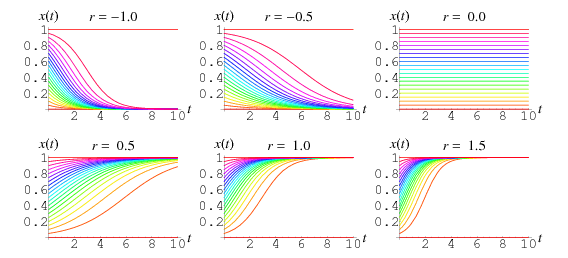
\includegraphics[scale=0.5]{./img/LogisticEquation.png}
    \caption{Logistic Equations}
\end{figure}

\end{enumerate}

\section{Systems of Differential Equations}

Just like in conventional algebra problems, we can have systems of differential equations. A solution of a system of two differential equations is a pair of functions $x(t)$ and $y(t)$ that satisfy both equations.

The resulting equation can also be though of as a three dimensional solution in the form $(x(t), y(t)) = t$.

If one or more functions are dependent on other functions, then we call them coupled. Otherwise we call them decoupled.
\[
\begin{aligned}
\text{Coupled}
\begin{cases}
y\prime = xy\\
x\prime = yx
\end{cases}\\
\text{Decoupled}
\begin{cases}
y\prime = yt\\
x\prime = xt
\end{cases}
\end{aligned}
\]

    \subsection{Autonomous First Order System}
    Autonomous systems are not dependent on $t$, so we can treat them a little differently. For these equations we can use a phase plane, vector field, and the trajectory of the solution.

    The functions $x(t)$ and $y(t)$ can give us a parametric curve. This means that at any given point on the curve, we also have a tangent vector given by $\frac{dy}{dt}$ and$\frac{dx}{dt}$.

    Every solution of a system we call a state of the system, and the collection of all the trajectories and states is called a phase portrait.

    An equilibrium point for this two dimensional system is an $(x,y)$ point where
    \[
    \frac{dy}{dt} = 0 = \frac{dx}{dt}
    \]

    \subsection{Graphical Methods for Solving}
    Sketching is a pain in the ass\dots Therefore there are a couple tricks that we can use to make our lives easier.

    We can use nullclines to more easily draw the solutions. Nullclines are an adaptation of previously mentioned isoclines \eqref{sec:visde}. A V nullcline is an isocline of vertical slopes where $x\prime = 0$. An H nullcline is an isocline of horizontal slopes where $y\prime = 0$. Equilibria occurs at the point where these two nullclines intersect.

    Note, when existence and uniqueness hold for an autonomous system, phase plane trajectories never cross.

    \begin{figure}[ht]\label{fig:visrep}
    \centering
        \begin{subfigure}[b]{0.4\textwidth}
            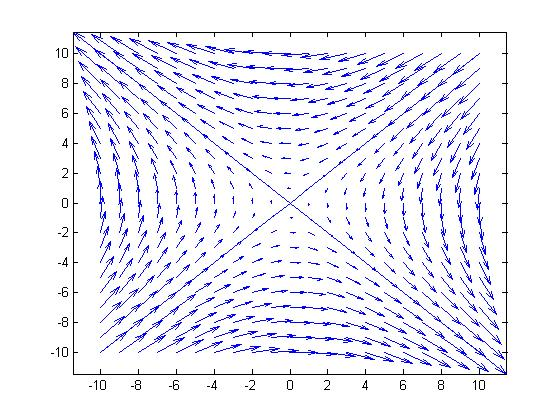
\includegraphics[scale=0.25]{./img/vectorfield.png}
            \caption{Vector Field}
        \end{subfigure}
        \begin{subfigure}[b]{0.4\textwidth}
            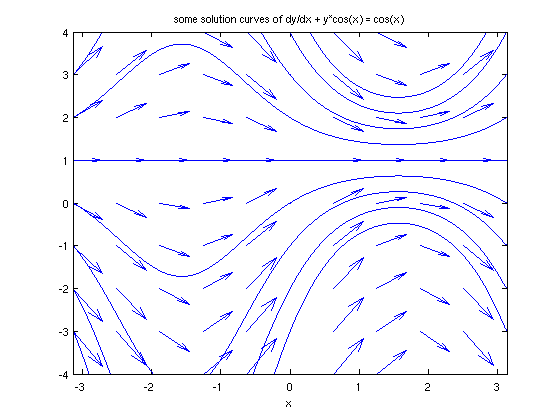
\includegraphics[scale=0.25]{./img/solutioncurves.png}
            \caption{Solution Curves}
        \end{subfigure}
    \caption{Visual Representations}
    \end{figure}

    \subsection{Quick Sketching Outline for Phase Portraits}
    \begin{enumerate}
    \item Nullclines and Equilibria
        \begin{itemize}
        \item Where $x\prime = 0$, slopes are vertical.
        \item Where $y\prime = 0$, slopes are horizontal.
        \item Where $x\prime = y\prime = 0$, we have equilibria.
        \end{itemize}
    \item Left-Right Directions
        \begin{itemize}
        \item Where $x\prime$ is positive, arrows point right.
        \item Where $x\prime$ is negative, arrows point left.
        \end{itemize}
    \item Up-Down Directions
        \begin{itemize}
        \item Where $y\prime$ is positive, arrows point up.
        \item Where $y\prime$ is negative, arrows point down.
        \end{itemize}
    \item Check Uniqueness\\
    Where phase plane trajectories do not cross, we have uniqueness.
    \end{enumerate}

    \subsection{Applications of Systems of Differential Equations}
        \subsubsection{Predator-Prey Assumptions}
        In the absence of foxes, the rabbit population will grow with the Malthusian Growth Law:
        \[
        \frac{dR}{dt} = a_R R, a_R > 0
        \]
        In the absence of rabbits, the fox population will die off according to the law:
        \[
        \frac{dF}{dtt} = -a_F F, a_F > 0
        \]
        When both foxes and rabbits are present, the number of interactions is $\propto$ the product of the population sizes, with inverse behavior. Thus we can get the Lotka-Volterra Equations for the predator prey model:

        \begin{equation}\label{eq:LVeq}
        \begin{cases}
        \frac{dR}{dt} = a_R R - c_R RF\\
        \frac{dF}{dt} = -a_F F - c_F RF
        \end{cases}
        \end{equation}

\section{Matrices}
    Using matrices enables us to do more complex operations on systems of equations, as well as other numbers and functions.

    \subsection{Definitions}
    A matrix is a rectangular array of elements arranged in rows and columns.

    \begin{equation}\label{eq:matrixdef}
    \mathbf{A} =
    \left[ \begin{matrix}
        a_1 & a_2 & a_3 & \cdots & a_n\\
        b_1 & b_2 & b_j & \cdots & b_n\\
        c_1 & c_2 & c_3 & \cdots & c_n\\
        \vdots & \vdots & \vdots & \ddots & \vdots\\
        m_1 & m_2 & m_3 & \cdots & m_n\\
    \end{matrix} \right]
    \end{equation}

    We can also describe these matrices by saying it has order $m \times n$ where $m$ and $n$ are the row and column sizes respectively. Two matrices are equal if they have the same $m$ and $n$ and the values contained are equal. We can also have matrices with orders $m \times 1$ or $n \times 1$ which are called column and row vectors.

    If all entries are 0, we call it a zero matrix; however if all entries but the diagonal are zero, this is called an diagonal matrix. These diagonal number are called diagonal elements. A special diagonal matrix is the identity matrix, which is formed when the diagonal elements are ones.

    \begin{equation}\label{eq:id_matrix}
        \left[ \begin{array}{cccc}
        1 & 0 & \cdots & 0\\
        0 & 1 & \cdots & 0\\
        \vdots & \vdots & 1 & \vdots\\
        0 & 0 & \cdots & 1\\
        \end{array} \right]
    \end{equation}

    \subsection{Addition and Multiplication}
    Most of the basic mathematical operations also apply to matrices. When adding two matrices, just add the components, when multiplying by a scalar, multiply each component by the scalar.

    Multiplication of two matrices is a little different however. When multiplying two matrices labeled $\mathbf{A}$ and $\mathbf{B}$ the steps are represented as follows.

    \begin{center}
        \textit{Each new element in the matrix is a result of the dot product between the corresponding row and column matrices.}
    \end{center}
    \begin{equation}\label{eq:matrixmultiplication}
    \begin{aligned}
        \mathbf{A}=
        \left[\begin{matrix}
        A_{11} & A_{12} & \cdots & A_{1m} \\
        A_{21} & A_{22} & \cdots & A_{2m} \\
        \vdots & \vdots & \ddots & \vdots \\
        A_{n1} & A_{n2} & \cdots & A_{nm} \\
        \end{matrix}\right]\\
        \quad\mathbf{B}=
        \left[\begin{matrix}
        B_{11} & B_{12} & \cdots & B_{1p} \\
        B_{21} & B_{22} & \cdots & B_{2p} \\
        \vdots & \vdots & \ddots & \vdots \\
        B_{m1} & B_{m2} & \cdots & B_{mp} \\
        \end{matrix}\right]\\
        \mathbf{A}\mathbf{B}=
        \left[\begin{matrix}
        A_1 \cdot B_1 & A_2 \cdot B_1 & \cdots & A_3 \cdot B_1 \\
        A_2 \cdot B_1 & A_2 \cdot B_2 & \cdots & A_2 \cdot B_3 \\
        \vdots & \vdots & \ddots & \vdots \\
        A_m \cdot B_1 & A_m \cdot B_2 & \cdots & A_m \cdot B_n \\
        \end{matrix}\right]
    \end{aligned}
    \end{equation}

    \subsection{Matrix Transposition}
    We can flip a matrix diagonally so that its columns become rows and its rows become columns. We call this the transpose of the matrix, written $\mathbf{A}^T$.

        \subsubsection{Example}
        \[
        \text{If } \mathbf{A} = \left[ \begin{array}{cc}
            1 & 2\\
            3 & 4\\
            5 & 6\\
        \end{array} \right] \text{ Then } \mathbf{A}^T
        \left[ \begin{array}{ccc}
            1 & 3 & 5\\
            2 & 4 & 6\\
        \end{array} \right]
        \]

        \subsubsection{Properties}
        \begin{itemize}
            \item ${(\ma^T)}^T = \ma$
            \item ${(\ma + \mb)}^T = \ma^T + \mb^T$
            \item ${(k \ma)}^T = k\ma^T$ for any scalar $k$.
            \item ${(\ma \mb)}^T = \ma^T \mb^T$
        \end{itemize}

    \subsection{Vectors as Special Matrices}
    For a given vector in $\mathbb{R}^n$, we can write

    \[
        \vec{x} =
        \left[\begin{matrix}
        x_1\\
        x_2\\
        \vdots\\
        x_n
        \end{matrix}\right] \text{ and }
        \vec{y} =
        \left[\begin{matrix}
        y_1\\
        y_2\\
        \vdots\\
        y_n
        \end{matrix}\right]
    \]
    We can also find the dot product of two matrices represented in this form using rules for matrix multiplication. Two vectors are orthogonal if their dot product is zero (See my Calculus III Notes, section 2, for more information).

    The absolute value of one of these vectors is equal to the matrix dotted with itself and square-rooted.

    \begin{equation}\label{eq:matrix_abs_val}
        ||\vec{v}|| \equiv \sqrt{\vec{v} \cdot \vec{v} }
    \end{equation}

\section{Matrices and Systems of Linear Equations}
Up until this point we've been solving systems of linear equations through fiddling with them (solving for different variables, etc.) until we get an answer. Using matrices we can solve them a lot more effectively. Not only that, but any process we use will turn the matrix into an equivalent system of equations, i.e., one that has the same solutions.

We can have systems of linear equations represented in matrices, and if all equations are equal to zero, the system is homogeneous. The solution is defined as the point in $\mathbb{R}^n$ whose coordinates solve the system of equations.

We have a couple of methods to solve systems of linear equations when they are in matrix form, but first we need to define a couple different terms and operations.

    \subsection{Augmented Matrix}
    An augmented matrix is where two different matrices are combined to form a new matrix.

    \begin{equation}\label{eq:augmented_matrix}
    \begin{aligned}
        \mathbf{[A|b]}=
        \left[\begin{array}{cccc|c}
        A_{11} & A_{12} & \cdots & A_{1m} & b_1\\
        A_{21} & A_{22} & \cdots & A_{2m} & b_2\\
        \vdots & \vdots & \ddots & \vdots & \vdots\\
        A_{n1} & A_{n2} & \cdots & A_{nm} & b_n\\
        \end{array}\right]\\
    \end{aligned}
    \end{equation}

    This is usually used to show the coefficients of the variables in a system of equations as well as the constants they are equal to.

    \subsection{Elementary Row Operations}
    We have a couple of different options to manipulate augmented matrices, which are as follows.

    \begin{itemize}
        \item Interchange row $i$ and $i$
            \[ R^*_i = R_j, R^*_j = R_i \]
        \item Multiply row $i$ by a constant.
            \[ R^*_i = cR_i \]
        \item Leaving $j$ untouched, add to $i$ a constant times $j$.
            \[ R^*_i = R_i + cR_j \]
    \end{itemize}

    These are handy when dealing with matrices and trying to obtain Reduced Row Echelon Form \eqref{sec:RREF}.

    \subsection{Reduced Row Echelon Form}\label{sec:RREF}
    When dealing with systems of linear equations in augmented matrix form we need to get it to a solution, which can be found with Reduced Row Echelon Form (RREF). This form looks similar to the following.

    \begin{equation}\label{eq:rref}
    \begin{aligned}
        \mathbf{[A|b]}=
        \left[\begin{array}{ccc|c}
        1 & 0 & 0 & b_1\\
        0 & 1 & 0 & b_2\\
        0 & 0 & 1 & b_3\\
        \end{array}\right]\\
    \end{aligned}
    \end{equation}

    This can be characterized by the following:

    \begin{itemize}
        \item $0$ rows are at the bottom.
        \item Leftmost non-zero entry is $1$, also called the pivot (or leading 1).
        \item Each pivot is further to the right than the one above.
        \item Each pivot is the only non-zero entry in its column.
    \end{itemize}

    A less complete process gives us row echelon form, which allows for nonzero entries are allowed above the pivot.

    \subsection{Gauss Jordan Reduction}
    This procedure will let us solve any given matrix/linear system. The steps are as follows.

    \begin{enumerate}
        \item Given a system $A\vec{x} = \vec{b}$
        \item Form augmented matrix $[A|b]$
        \item Transform to RREF \eqref{sec:RREF} using elementary row operations.
        \item The linear matrix formed by this process has the same solutions as the initial system, however it is much easier to solve.
    \end{enumerate}

    \subsection{Existence and Uniqueness}
    If the RREF has a row that looks like:
    \[
        [0, 0, 0, \cdots, 0 | k]
    \]
    where $k$ is a non-zero constant, then the system has no solutions. We call this inconsistent.

    If the system has one or more solutions, we call it consistent.

    In order to be unique, the system needs to be consistent.
        \begin{itemize}
            \item If every column is a pivot, the there is only one solution (unique solution).
            \item Else If most columns are pivots, there are multiple solutions (possibly infinite).
            \item Else the system is inconsistent.
        \end{itemize}

    \subsection{Superposition, Nonhomogeneous Principle, and RREF}
    For any nonhomogeneous linear system $\mathbf{A}\vec{x} = \vec{b}$, we can write the solutions as:
    \[
        \vec{x} = \vec{x}_h + \vec{x}_p
    \]
    Where $\vec{x}_h$ represents vectors in the set of homogeneous solutions, and $\vec{x}_p$ is a particular solution to the original equation.

    We can use RREF to find $\vec{x}_p$, and then, using the same RREF with $\vec{b}$ replaced by $\vec{0}$, find $\vec{x}_h$.

    The rank of a matrix $r$ equals the number of pivot columns in the RREF. If $r$ equals the number of variables, there is a unique solution. Otherwise if there is less, then it is not unique.

    \subsection{Inverse of a Matrix}
    When given a system of equations like:
    \[
        \begin{cases}
            x + y = 1\\
            4x + 5y = 6
        \end{cases}
    \]
    we can rewrite it in the form:
    \[
        \left[\begin{array}{cc}
        1 & 1\\
        4 & 5
        \end{array}\right]
        \left[\begin{array}{c}
            x\\
            y
        \end{array}\right] =
        \left[\begin{array}{c}
            1\\
            6
        \end{array}\right]
    \]
    For this sort of matrix, we can find the inverse which is defined as the matrix that, when multiplied with the original, equals an Identity Matrix. In other words:
    \[ A^{-1}A = AA^{-1} = I \]

        \subsubsection{Properties}
        \begin{itemize}
        \item ${( A^{-1})}^{-1} = A$
        \item $A$ and $B$ are invertible matrices of the same order if $\left(AB\right) = A^{-1}B^{-1}$
        \item If $A$ is invertible, then so is $A^T$ and $\left(A^{-1}\right)^T = \left(A^T\right)^{-1}$
        \end{itemize}

        \subsubsection{Inverse Matrix by RREF}
        For an $n\times n$ matrix $A$, the following procedure either produces $A^{-1}$, or proves that it's impossible.

        \begin{enumerate}
        \item Form the $n \times 2n$ matrix $M=\left[A|I\right]$
        \item Transform $M$ into its RREF, $R$.
        \item If the first $n$ columns produce an Identity Matrix, then the last $n$ are its inverse. Otherwise $A$ is not invertible.
        \end{enumerate}

    \subsection{Invertibility and Solutions}
    The matrix vector equation $A\mathbf{x} = b$ where $A$ is an $n \times n$ matrix has:
        \begin{itemize}
        \item A unique solution $x=A^{-1} b$ if and only if $A$ is invertible.
        \item Either no solutions or infinitely many solutions if $A$ is not invertible.
        \end{itemize}

    For the homogeneous equation $A \mathbf{x} = 0$, there is always one solution, $x=0$ called the trivial solution.

    Let $\ma$ be an $n \times n$ matrix. The following statements apply.
    \begin{itemize}
        \item $\ma$ is an invertible matrix.
        \item $\ma^T$ is an invertible matrix.
        \item $\ma$ is row equivalent to $I_n$.
        \item $\ma$ has $n$ pivot columns.
        \item The equation $\ma \vec{x} = \vec{0}$ has only the trivial solution, $\vec{x}=\vec{0}$.
        \item The equation $\ma \vec{x} = \vec{0}$ has a unique solution for every $\vec{b}$ in $\mathbb{R}^n$.
    \end{itemize}

    \subsection{Determinants and Cramer's Rule}
    The determinant of a square matrix is a scalar number associated with that matrix. These are very important.

        \subsubsection{$2 \times 2$ Matrix}\label{subsubsec:22mat}
        To find the determinant of a $2 \times 2$ matrix, the determinant is the diagonal products subtracted. This process is demonstrated below.

        \begin{equation}\label{eq:22det}
        \begin{aligned}
            A =
            \left[\begin{array}{cc}
                a_{11} & a_{12}\\
                a_{21} & a_{22}
            \end{array}\right]\\
            \left| A \right| = a_{22} \cdot a_{11} - a_{12} \cdot a_{21}
        \end{aligned}
        \end{equation}

        \subsubsection{Definitions}
        Every element of a $n \times n$ matrix has an associated minor and cofactor.

        \begin{itemize}
        \item Minor $\to$ A $(n - 1) \times (n - 1)$ matrix obtained by deleting the $i$th row and $j$th column of $A$.
        \item Cofactor $\to$ The scalar $C_{ij} = (C - 1)^{i+j} \left| M_{ij} \right|$
        \end{itemize}

        \subsubsection{Recursive Method of an $n \times n$ matrix $A$}
        We can now determine a recursive method for any $n \times n$ matrix.

        Using the definitions declared above, we use the recursive method that follows.

        \begin{equation}\label{eq:detrec}
        \left| A \right| = \sum_{j=1}^n a_{ij} C_{ij}
        \end{equation}

        Find $j$ and then finish with the rules for the $2 \times 2$ matrix defined above in \eqref{subsubsec:22mat}.

        \subsubsection{Row Operations and Determinants}
        Let $A$ be square.

        \begin{itemize}
        \item If two rows of $A$ are exchanged to get $B$, then $|B| = -|A|$.
        \item If one row of $A$ is multiplied by a constant $c$, and then added to another row to get $B$, then $|A| = |B|$.
        \item If one row of $A$ is multiplied by a constant $c$, then $|B| = c|A|$.
        \item If $|A| = 0$, $A$ is called singular.
        \end{itemize}

        For an $n \times n$ $A$ and $B$, the determinant $|AB|$ is given by $|A||B|$.

        \subsubsection{Properties of Determinants}
        \begin{itemize}
        \item If two rows of $\ma$ are interchanged to equal $\mb$, then
            \[ | \mb | = - | \ma | \]
        \item If one row of $\ma$ is multiplied by a constant $k$, and then added to another row to produce matrix $\mb$, then
            \[ | \mb | = | \ma | \]
        \item If one row of $\ma$ is multiplied by $k$ to produce matrix $\mb$, then
            \[ | \mb | = k | \ma | \]
        \item If $|AB| = 0$, then either $|A|$ or $|B|$ must be zero.
        \item $|A^T| = A$
        \item If $| \ma | \neq 0$, then $| \ma^{-1} | = \frac{1}{|\ma |}$.
        \item If $A$ is an upper or lower triangle matrix\footnote{A triangle matrix is one where either the lower or upper half is zero, e.g. $\left[\begin{array}{cccc}1 & 0 & 0 & 0\\1 & 1 & 0 & 0\\1 & 1 & 1 & 0\\1 & 1 & 1 & 1\end{array}\right]$.}, then the determinant is the product of the diagonals.
        \item If one row or column consists of only zeros, then $|A| = 0$.
        \item If two rows or columns are equal, then $|A|=0$.
        \item $A$ is invertible.
        \item $A^T$ is also invertible.
        \item $A$ has $n$ pivot columns.
        \item $|A| \neq 0$
        \item If $|A| = 0$ it is called singular, otherwise it is nonsingular.
        \end{itemize}

        \subsubsection{Cramer's Rule}
        For the $n \times n$ matrix $A$ with $|A| \neq 0$, denote by $A_i$ the matrix obtained from $A$ by replacing its $i$th column with the column vector $\mathbf{b}$. Then the $i$th component of the solution of the system is given by:

        \begin{equation}\label{eq:cramer}
            x_i = \frac{|A_i|}{|A|}
        \end{equation}


\section{Vector Spaces and Subspaces}
A vector space $\mathcal{V}$ is a non-empty collection of elements that we call vectors, for which we can define the operation of vector addition and scalar multiplication:
    \begin{enumerate}
    \item Addition: $\vec{x} + \vec{y}$
    \item Scalars: $c \vec{x}$ where $c$ is a constant.
    \end{enumerate}
that satisfy the following properties:
    \begin{enumerate}
    \item $\vec{x} + \vec{y} \in \mathcal{V}$
    \item $c \vec{x} \in \mathcal{V}$
    \end{enumerate}

which can be condensed into a single equation:
\[
    c\vec{x} + d\vec{y} \in \mathcal{V}
\]
which is called closure under linear combinations.

    \subsection{Properties}
    We have the properties from before, as well as new ones.

    \begin{enumerate}
    \item $\vec{x} + \vec{y} \in \mathcal{V} \leftarrow $ Addition
    \item $c \vec{x} \in \mathcal{V} \leftarrow $ Scalar Multiplication
    \item $\vec{x} + \vec{0} = \vec{x} \leftarrow $ Zero Element
    \item $\vec{x} + (-\vec{x}) = (-\vec{x}) + \vec{x} = \vec{0} \leftarrow $ Additive Inverse
    \item $(\vec{x} + \vec{y}) + \vec{z} = \vec{x} + (\vec{y} + \vec{z}) \leftarrow$ Associative Property
    \item $\vec{x} + \vec{y} = \vec{y} + \vec{x} \leftarrow $ Commutativity
    \item $1 \cdot \vec{x} = \vec{x} \leftarrow$ Identity
    \item $c (\vec{x} + \vec{y}) = c\vec{x} + c\vec{y} \leftarrow $ Distributive Property
    \item $(c + d) \vec{x} = c\vec{x} + d\vec{x} \leftarrow $ Distributive Property
    \item $c(d\vec{x}) = (cd)\vec{x} \leftarrow $ Associativity
    \end{enumerate}

    \subsection{Vector Function Space}
    A vector function space is just a unique vector space where the elements of the space are functions.

    Note, the solutions to linear and homogeneous differential equations form vector spaces.

        \subsubsection{Closure under Linear Combination}
        \begin{equation}\label{eq:funcspace_closure}
            c \vec{x} + d \vec{y} \in \mathbb{V} \text{ whenever } \vec{x}, \vec{y} \in \mathbb{V} \text{ and } c, d \in \mathbb{R}
        \end{equation}

        \subsubsection{Prominent Vector Function Spaces}
        \begin{itemize}
            \item $\mathbb{R}^2 \to$ The space of all ordered pairs.
            \item $\mathbb{R}^3 \to$ The space of all ordered triples.
            \item $\mathbb{R}^n \to$ The space of all ordered $n$-tuples.
            \item $\mathbb{P} \to$ The space of all polynomials.
            \item $\mathbb{P}_n \to$ The space of all polynomials with degree $\le n$.
            \item $\mathbb{M}_{mn} \to$ The space of all $m \times n$ matrices.
            \item $\mathbb{C}(I) \to$ The space of all continuous functions on the interval $I$ (open, closed, finite, and infinite).
            \item $\mathbb{C}^n(I) \to$ Same as above, except with $n$ continuous derivatives.
            \item $\mathbb{C}^n \to$ The space of all ordered $n$-tuples of complex numbers.
        \end{itemize}

    \subsection{Vector Subspaces}
    \textbf{Theorem:} A non-empty subset $\mathbb{W}$ of a vector space $\mathbb{V}$ is a subspace of $\mathbb{V}$ if it is closed under addition and scalar multiplication:
    \begin{itemize}
        \item If $\vec{u}, \vec{v} \in \mathbb{W}$, than $\vec{u} + \vec{V} \in \mathbb{W}$.
        \item If $\vec{u} \in \mathbb{W}$ and $c \in \mathbb{R}$, than $c\vec{u} \in \mathbb{W}$.
    \end{itemize}

    We can rewrite this to be more efficient:

    \begin{equation}\label{eq:subspace_closure}
        \text{If } \vec{u}, \vec{v} \in \mathbb{W} \text{ and } a, b \in \mathbb{R}, \text{ than } a\vec{u} + b\vec{v} \in \mathbb{W}.
    \end{equation}

    Note, vector space does not imply subspace. All subspaces are vector spaces, but not all vector spaces are subspaces.

    To determine if it is a subspace, we check for closure with the above theorem.

    There are only a couple subspaces for $\mathbb{R}^2$:
    \begin{itemize}
        \item The zero subspace $\left\{ (0, 0) \right\}$.
        \item Lines passing through the origin.
        \item $\mathbb{R}^2$ itself.
    \end{itemize}

    We can call the zero and the set $\mathbb{V}$ themselves trivial subspaces, calling the subspace of lines passing through the origin the only non-trivial subspace in $\mathbb{R}^2$.

    We can classify $\mathbb{R}^3$ similarly:
    \begin{itemize}
    \item Trivial:
        \begin{itemize}
        \item Zero subspace
        \item $\mathbb{R}^3$
        \end{itemize}
    Non-Trivial
        \begin{itemize}
        \item Lines that contain the origin.
        \item Places that contain the origin.
        \end{itemize}
    \end{itemize}

        \subsubsection{Examples}
        \begin{itemize}
        \item The set of all even functions.
        \item The set of all solutions to $y\prime\prime\prime - y\prime\prime t + y = 0$.
        \item $\{P \in \mathbb{P}; P(2) = P(3)\}$
        \end{itemize}

\section{Span, Basis and Dimension}
Given one or more vectors in a vector space, we can create more vectors through addition and scalar multiplication. These vectors that result from this process are called linear combinations.

    \subsection{Span}
    The span of a set $\{\vec{v}_1, \vec{v}_2, \ldots, \vec{v}_n\}$ of vectors in a vector space $\mathbb{V}$, denoted by Span$\{\vec{v}_1, \vec{v}_2, \ldots, \vec{v}_n\}$ is the set of all linear combinations of the vectors.

        \subsubsection{Example}
    \[
        \begin{aligned}
            \text{For example, If } \vec{u} = \left[ \begin{array}{c} 3\\2\\0 \end{array} \right] \text{ and } \vec{v} = \left[ \begin{array}{c} 0\\2\\2 \end{array} \right]\\
            \text{Then we can write their span as }\\
            a\vec{u} + b\vec{v} = a\left[ \begin{array}{c} 3\\2\\0 \end{array} \right] + b\left[ \begin{array}{c} 0\\2\\2 \end{array} \right] = \left[ \begin{array}{c} 3a\\2a+2b\\2b \end{array} \right]
        \end{aligned}
    \]

    \subsection{Spanning Sets in $\mathbb{R}^n$}
    A vector $\vec{b}$ in $\mathbb{R}^n$ is in Span$\{\vec{v}_1, \vec{v}_2, \ldots, \vec{v}_n\}$ where $\{\vec{v}_1, \vec{v}_2, \ldots, \vec{v}_n\}$ are vectors in $\mathbb{R}^n$, provided that there is at least one solution of the matrix-vector equation $A\vec{x} = \vec{b}$, where $A$ is the matrix whose column vectors are $\{\vec{v}_1, \vec{v}_2, \ldots, \vec{v}_n\}$.

    \subsection{Span Theorem}
    For a set of vectors $\{\vec{v}_1, \vec{v}_2, \ldots, \vec{v}_n\}$ in vector space $\mathbb{V}$, Span$\{\vec{v}_1, \vec{v}_2, \ldots, \vec{v}_n\}$ is subspace of $\mathbb{V}$.

    \subsection{Column Space}
    For any $m \times n$ matrix $A$, the column space, denoted Col $A$, is the span of the column vectors of $A$, and is a subspace of $|mathbb{R}^n$.

    \subsection{Linear Independence}
    A set $\{\vec{v}_1, \vec{v}_2, \ldots, \vec{v}_n\}$ of vectors in vector space $\mathbb{V}$ is linearly independent if no vector of the set can be written as a linear combination of the others. Otherwise it is linearly dependent.

    This notion of linear independence also carries over to function spaces. A set of vector functions $\{\vec{v}_1, \vec{v}_2, \ldots, \vec{v}_n\}$ in a vector space $\mathbb{V}$ is linearly independent on an interval $I$ if for all $t$ in $I$ the only solution of
    \[
    c_1 \vec{v}_1 + c_2 \vec{v}_2 + \cdots + c_n \vec{v}_n = \vec{0}
    \]
    for $(c_1, c_2, \ldots, c_n \in \mathbb{R})$ is $c_i = 0$ for all $i$.

    If for any value $t_0$ of $t$ there is any solution with $c_i \neq \vec{0}$, the vector functions are linearly dependent.


        \subsubsection{Testing for Linear Independence}
        \begin{enumerate}
        \item \begin{enumerate}
            \item Put the system in matrix-vector form:
                \[
                \left[ \begin{array}{cccc}
                    \uparrow & \uparrow & \cdots & \uparrow\\
                    \vec{v}_1 & \vec{v}_2 & \cdots & \vec{v}_n\\
                    \downarrow & \downarrow & \cdots & \downarrow\\
                \end{array} \right] \left[ \begin{array}{c}
                    c_1\\
                    c_2\\
                    \vdots\\
                    c_n
                \end{array}\right] = \vec{0}
                \]
            \item Analyze Matrix:\\
                The column vectors of $A$ are linearly independent if and only if the solution $\vec{x} = \vec{0}$ is unique, which means $c_i = 0$ for all $i$.\\
                Any of the following also satisfy this condition for a unique solution:
                    \begin{itemize}
                        \item $A$ is invertible.
                        \item $A$ has $n$ pivot columns.
                        \item $|A| \neq 0$
                    \end{itemize}
            \end{enumerate}
        \item Suppose we have a set of vectors $\vec{v}$.
            \[
                \left\{ \vec{v}_1, \vec{v}_2, \ldots, \vec{v}_n \right\} \in \mathbb{R}^n, \dim(\vec{v})=m
            \]
            Then the set $\vec{v}$ is linearly dependent if $n>m$ where $n$ is the number of elements in $\vec{v}$. \textit{Note, this cannot prove the opposite. It only goes one way.}
            \[
                \left\{
                \left(\begin{array}{c}
                    1\\
                    2\\
                    3
                \end{array}\right),
                \left(\begin{array}{c}
                    4\\
                    5\\
                    6
                \end{array}\right),
                \left(\begin{array}{c}
                    0\\
                    1\\
                    0
                \end{array}\right),
                \left(\begin{array}{c}
                    1\\
                    -3\\
                    7
                \end{array}\right)
                \right\} \text{Is dependent}
            \]
        \item Columns of $A$ are linearly independent if and only if $\mathbf{A}\vec{x} = \vec{0}$ has only the trivial solutions of $n$.
        \end{enumerate}

        \subsubsection{Linear Independence of Functions}
        One way to check a set of functions is to consider them as a one dimensional vector.
        \[
            \vec{v}_i (t) = f_n(t)
        \]
        Another method is the Wronskian:
        \begin{equation}\label{eq:wronskian}
        \begin{aligned}
            \text{To find the Wronskian of functions } f_1, f_2, \ldots, f_n \text{ on } I:\\
            W[f_1, f_2, \ldots, f_n] = \left[ \begin{array}{cccc}
                    f_1 & f_2 & \cdots & r_n\\
                    f^{'}_1 & f^{'}_2 & \cdots & r^{'}_n\\
                    \vdots & \vdots & \ddots & \vdots\\
                    f^{n-1}_1 & f^{n-1}_2 & \cdots & r^{n-1}_n\\
            \end{array} \right]
        \end{aligned}
        \end{equation}
        If $W \neq 0$ for all $t$ on the interval $I$, where $f_1, f_2, \ldots, f_n$ are defined, then the function space is a linearly independent set of functions on $I$.

    \subsection{Basis of a Vector Space}
    The set $\{\vec{v}_1, \vec{v}_2, \ldots, \vec{v}_n\}$ is a basis for vector space $\mathbb{V}$ provided that

    \begin{itemize}
        \item $\{\vec{v}_1, \vec{v}_2, \ldots, \vec{v}_n\}$ is linearly independent.
        \item Span$\{\vec{v}_1, \vec{v}_2, \ldots, \vec{v}_n\} = \mathbb{V}$
    \end{itemize}

        \subsubsection{Standard Basis for $\mathbb{R}^n$}
        \begin{equation}\label{eq:basis_for_rn}
        \begin{aligned}
            \{\vec{e}_1, \vec{e}_2, \ldots, \vec{e}_n\}\\
            \text{where}\\
            \vec{e}_1 = \left[ \begin{array}{c}
                1\\
                0\\
                0\\
                \vdots\\
                0
            \end{array}\right],
            \vec{e}_2 = \left[ \begin{array}{c}
                0\\
                1\\
                0\\
                \vdots\\
                0
            \end{array}\right], \ldots,
            \vec{e}_n = \left[ \begin{array}{c}
                0\\
                0\\
                0\\
                \vdots\\
                1
            \end{array}\right]
        \end{aligned}
        \end{equation}
        are the column vectors of the identity matrix $I_n$.

        \subsubsection{Example}
        A vector space can have different bases.

        The standard basis for $\mathbb{R}^n$ is:
        \[
        \{\vec{e}_1, \vec{e}_2\} \text{ for } \vec{e}_1 =
        \left[ \begin{array}{c}
        1\\
        0
        \end{array}\right] \text{ and } \vec{e}_2
        \left[ \begin{array}{c}
        0\\
        1
        \end{array}\right] \text{ giving }
        \left\{ \left[ \begin{array}{c}
        1\\
        0
        \end{array}\right],
        \left[ \begin{array}{c}
        0\\
        1
        \end{array}\right]\right\}
        \]

        But another basis for $\mathbb{R}^2$ is given by:

        \[
        \left\{ \left[ \begin{array}{c}
        2\\
        1
        \end{array}\right],
        \left[ \begin{array}{c}
        1\\
        2
        \end{array}\right]\right\}
        \]
    \subsection{Dimension of the Column Space of a Matrix}
    Essentially, the number of vectors in a basis.

        \subsubsection{Properties}
        \begin{itemize}
            \item The pivot columns of a matrix $A$ form a basis for Column $A$.
            \item The dimension of the column space, called the rank of $A$, is the number of pivot columns in $A$.
                \[
                    \text{rank } A = \dim(\text{Col}(A))
                \]
        \end{itemize}

        \subsubsection{Invertible Matrix Characterizations}
        Let $A$ be an $n \times n$ matrix. The following are true.
        \begin{itemize}
            \item $A$ is invertible.
            \item The column vector of $A$ is linearly independent.
            \item Every column of $A$ is a pivot column.
            \item The column vectors of $A$ form a basis for Col$(A)$.
            \item Rank $A = n$
        \end{itemize}
\section{Higher Order Linear Differential Equations}
The second order linear homogeneous equation \eqref{eq:2lde} is vital; it allows us to model a wide set of equations that are both found in nature, as well as purely theoretical.

    \begin{equation}\label{eq:2lde}
        m \ddot{x} + b \dot{x} + kx = f(t)
    \end{equation}

    Where $x$ is our given equation, $\dot{x}$ is the first derivative of $x$, and $\ddot{x}$ is the second derivative of $x$. $f(t)$ is any equation. The behavior of this second order differential equation will vary based on the values of $m, b, k$, and $f(t)$.

    \subsection{Harmonic Oscillators}
    Our established equation for second order differential equations can help model many different types of behavior found in nature.

        \subsubsection{The Mass-Spring System}
        Consider an object with mass $m$ on a table that is attached to a spring attached to wall. When the object is moved by an external force, we can model its behavior using Newton's Second Law of Motion: $F = m \ddot{x}$ where $F$ is the sum of the forces acting on the object.

        \begin{figure}[h!]
            \centering
            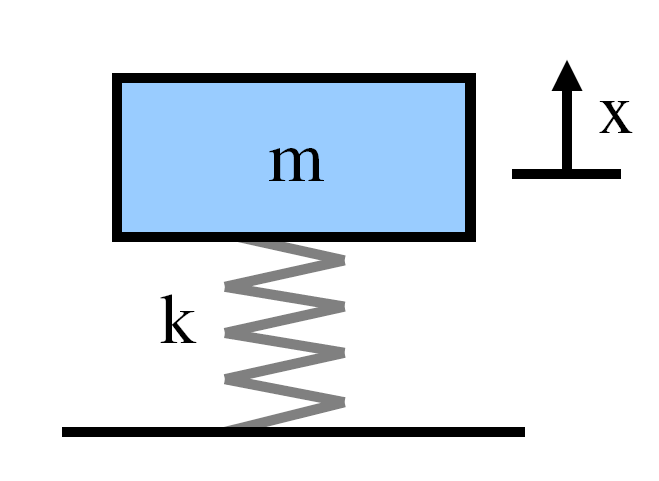
\includegraphics[scale=0.25]{./img/mass_spring.png}
            \label{fig:massspringsystem}
            \caption{Visual Representation of a Mass-Spring System}
        \end{figure}

        We have three different types of forces:

            \begin{itemize}
                \item \textbf{Restoring Force:} The restorative force of a spring is $\propto$ the amount of stretching/compression:
                    \[ F_{\text{restoring} } = -k x \]
                \item \textbf{Damping Force:} We also assume that friction exists, and therefore a damping force $\propto$ the velocity of the object:
                    \[ F_{\text{damping} } = -b \dot{x} \]
                    Where damping constant $b > 0$ and small for slick surfaces.
                \item \textbf{External Force:} We also allow for an external force to drive the motion:
                    \[ F_{\text{external} } = f(t) \]
            \end{itemize}

        Thus we get our equation for a Simple Harmonic Oscillator:

            \[ m \ddot{x} + b \dot{x} + kx = f(t) \]

            \begin{itemize}
                \item Constants $m>0, k>0, b>0$
                \item When $b=0$, the motion is called undamped. Otherwise it is damped.
                \item if $f(t)=0$, the equation is homogeneous and the motion is called unforced, undriven, or free. Otherwise it is forced, or driven.
            \end{itemize}

        \subsubsection{Solutions}
        When we say solution, we are referring to a solution that gives us $x$, in other words, the position of the mass at any given time $t$ as a function of $t$. Due to the inherent nature of derivatives, this may or may not have undetermined constants (often denoted as $[c_1, c_2, \dots, c_n]$) as will be set by initial values given (similar to first order differential equations).

        Later we will determine how to solve these equations fully, however a quick answer can be found by applying the following formulas. After learning the methods given ahead, be sure to come back and determine how these solutions were determined.

            \[ \begin{aligned}
                \text{Given Equation: } m \ddot{x} + kx = 0\\
                x(t) = c_1 \cos \left( \omega_0 t \right) + c_2 \sin \left( \omega_0 t \right)\\
                \omega_0 = \sqrt{\frac{k}{m} }
            \end{aligned} \]

        This gives us one form of the solution, however we can also find an alternate form:

            \[ x(t) = A \cos \left( \omega_0 t - \delta \right) \]

        Where
            \begin{itemize}
                \item Amplitude $A$ and phase angle $\delta$ (radians) are arbitrary constants determined by initial conditions.
                \item The motion has circular frequency $\omega_0 = \sqrt{\frac{k}{m} }$ (radians) per second, and a natural frequency $f_0 = \frac{\omega_0}{2 \pi}$
                \item The period $T$ (seconds) is $2 \pi \sqrt{\frac{m}{k} }$
                \item The above solution is a horizontal shift of $A \cos (\omega_0 t)$ with phase shift $\frac{\delta}{\omega_0}$.
            \end{itemize}

        To convert between the two forms, apply the following formulas.

            \[
                \begin{cases}
                    A = \sqrt{c_1^2 + c_2^2}\\
                    \tan \delta = \frac{c_2}{c_1}
                \end{cases}
                \begin{cases}
                    c_1 = A \cos \delta\\
                    c_2 = A \sin \delta
                \end{cases}
            \]

        To solve the Mass-Spring System with both damping and forcing as given by the following equation:

            \[
                m \ddot{x} + b\dot{x} + kx = F_0 \cos ( \omega_f t )
            \]

        we can apply the following formula. (Note, some concepts are explained later in the text, refer back if needed)

        \begin{enumerate}
            \item $x_h(t)$ has three possible solutions. See \eqref{sec:2deroots}.
            \item $x_p(t)$ can be assumed as
                \[ A \cos ( \omega_f t ) + B \sin ( \omega_f t )\]
                See \eqref{sec:2decoefficients}.
            \item \[ \omega_0 = \sqrt{\frac{k}{m} } \]
            \item \[ A = \frac{m (\omega_0^2 - \omega_f^2) F_0}{m^2{(\omega_0^2 - \omega_f^2)}^2 + {(b \omega_f)}^2} \]
            \item \[ B = \frac{b \omega_f F_0}{m^2{(\omega_0^2 - \omega_f^2)}^2 + {(b \omega_f)}^2} \]
        \end{enumerate}

        As you can see, this is a pain. Values $A$ and $B$ in particular are tedious to calculate. Despite this, as you'll see later, these methods can be easier than solving by hand.

        \subsubsection{Phase Planes}\label{sec:2depplane}
        For any autonomous second order differential equation

            \[ \ddot{x} = F(x, \dot{x}) \]

        the phase plane is the two dimensional graph with $x$ and $\dot{x}$ axes (which are the position and velocity respectively)\footnote{This concept of a phase plane is identical to the one introduced in \eqref{sec:visde} with the exception of $\dot{x}$ replacing $y$.}. This phase plane has a vector field with direction given by

            \[ \begin{cases}
                    H \to \frac{dx}{dt} = \dot{x}\\
                    V \to \frac{d\dot{x} }{dt} = \ddot{x}
                \end{cases} \]

        Trajectories can be formed by parametrically combining the vectors into a path. A graph showing these trajectories is called a phase portrait.

        The differential equation is also equivalent to the system of equations:

            \[ \begin{cases}
                    \dot{x} = y\\
                    \dot{y} = \ddot{x} = f(t) - \frac{k}{m} x - \frac{b}{m} y
                \end{cases} \]

        The biggest advantage with phase portraits is that is allows the user to solve the differential equation graphically, and not numerically. This can be much easier if done correctly.

    \subsection{Properties and Theorems}
    For the linear homogeneous, second-order differential equation

        \[
            y\prime\prime + p(t) y\prime + q(t)y = 0
        \]

    with $p$ and $q$ being continuous functions of $t$, there exists a two-dimensional vector space of solutions.

    Rewriting the above equation gives us

        \[
            y\prime\prime(t) \equiv f(t, y, y\prime) = -p(t) y\prime - q(t) y = 0
        \]

    which gives us the existence and uniqueness theorem for the second order equation.

        \begin{thm}[Existence and Uniqueness]\label{thm:2eau}
            Let $p(t)$ and $q(t)$ be continuous on $a, b$ containing $t_0$. For any $A$ and $B$ in $\mathbb{R}$, there exists a unique solution $y(t)$ defined on $(a, b)$ to the IVP
            \[
            y\prime\prime + p(t) y\prime + q(t)y = 0, y(t_0) = A, y\prime(t_0) = B
            \]
        \end{thm}

    A basis exists for the general second order equation.

        \begin{thm}[Solution Space]\label{thm:solutionspace}
            The solution space $S$ for a second order homogeneous differential equation has a Dimension of 2.
        \end{thm}

    For any linear second order homogeneous differential equation on $(a, b)$,

        \[
            y\prime\prime + p(t) y\prime + q(t)y = 0
        \]

    for which $p$ and $q$ are continuous on $(a, b)$, any two linearly independent solutions $\{y_1, y_2\}$ form a basis of the solutions space $S$, and every solution $y$ on $(a, b)$ can be written as

        \[
            y(t) = c_1 y_1(t) + c_2 y_2(t) \to (c_1, c_2) \in \mathbb{R}
        \]

    To generalize we can apply the same principle to $nth$ order differential equations.

        \begin{thm}[Existence and Uniqueness for $nth$ Order Differential Equations]\label{thm:neau}
        Let $p_1(t), p_2(t), \dots, p_n(t)$ be continuous functions on $(a, b)$ containing $t_0$. For any initial values $A_0, A_1, \dots, A_{n-1} \in \mathbb{R}$, there exists a unique solution $y(t)$ to the IVP
        \[
        \begin{aligned}
            y\prime\prime(tp_1(t)y^{n - 1}(t)) + p_1(t)y^{n - 1}(t) + p_2(t)y^{n - 2}(t) + \cdots + p_n(t)y(t) = 0\\
            y(t_0) = A_0, y\prime(t_0) = A_1, \dots, y^{n - 1}(t_0) = A_{n-1}
        \end{aligned}
        \]
    \end{thm}

    For $n$th order differential equations, our solution space theorem \eqref{thm:solutionspace} applies, just replace the term ``2'' and ``second'' with ``$n$'' and ``$n$th''.

    \subsection{Roots}\label{sec:2deroots}
    If given a second order equation in the form $a \ddot{y} + b \dot{y} + cy = 0$, we can use our previous definition of a first order differential equation to find an easier method of solving. At its core, this method consists of converting our given second order differential equation and converting it into a quadratic equation, using which we can solve for the homogeneous solution.

        \begin{equation}\label{eq:2de-quad}
            a \ddot{y} + b \dot{y} + cy = 0 \Leftrightarrow ar^2 + br + c = 0
        \end{equation}

    The resulting equation is called the characteristic equation. Solutions to this equation are called characteristic roots. Due to the nature of quadratic equations, there are three different possibilities for the solution:

        \begin{itemize}
            \item Two distinct real roots or zeros
            \item One real root (a double root)
            \item Two imaginary roots
        \end{itemize}

    These are summarized as follows.

        \begin{table}[ht]
            \centering
            \scalebox{0.9}{
            \begin{tabular}{| l | l | l |}
                \hline
                \textbf{Case One} & Real Unequal Roots & Overdamped Motion\\
                $\Delta > 0$ & $r_1, r_2 = \frac{-b \pm \sqrt{b^2 - 4ac} }{2a}$ & $y_h(t) = c_1 e^{r_1 t} + c_2 e^{r_2 t}$\\&&\\
                \hline
                \textbf{Case Two} & Real Repeated Root & Critically Damped Motion\\
                $\Delta = 0$ & $r = - \frac{b}{2a} $ & $y_h(t) = c_1 e^{r t} + c_2 t e^{r t}$\\&&\\
                \hline
                \textbf{Case Three} & Complex Conjugate Roots & Underdamped Motion\\
                $\Delta < 0$ & $r_1, r_2 = \alpha \pm \beta i$ & $y_h(t) = e^{\alpha t} \left( c_1 \cos \left(\beta t \right) + c_2 \sin \left( \beta t \right) \right)$\\
                & $\alpha = - \frac{b}{2a}, \beta = \frac{\sqrt{4ac - b^2} }{2a}$ &\\&&\\
                \hline
            \end{tabular} }
            \caption{Roots for Second Order Differential Equations in Characteristic Equation Form}
            \label{table:roots}
        \end{table}

    These methods allow us to generalize for higher order differential equations and find solutions that would be otherwise impossible.

    \subsection{Linear Independence}
    The Solution Space Theorem \eqref{thm:solutionspace} provides us with the number of solutions in a bases for an $n$th order homogeneous differential equation ($n$).

    \begin{itemize}
        \item Starting with $m$ solutions for the $n$th order case, if $m > n$ the solutions can no be independent.
        \item If $m=n$, we must test using the concepts from before.
        \item If $m < n$, the set does not span the space.
    \end{itemize}

        \subsubsection{Wronskian}
        The Wronskian also tells us about the linear independence of a set of functions. This Wronskian is identical to the Wronskian previously defined \eqref{eq:wronskian}.

        Suppose $\{y_1, y_2, \dots, y_n \}$ is a set of solutions of an $n$th order homogeneous differential equation.

            \[
                L(y) = a_n(t)y^n + a_{n-1}(t)y^{n-1} + \cdots + a_1 (t)y\prime + a_0 (t)y = 0
            \]
            \begin{enumerate}
                \item If $W[y_1, y_2, \dots, y_n] \neq 0$ at any point on $(a, b)$, then the set is linearly independent.
                \item If $W[y_1, y_2, \dots, y_n] = 0$ at every point on $(a, b)$, then the set is linearly dependent.
            \end{enumerate}

    \subsection{Undetermined Coefficients}\label{sec:2decoefficients}
    Let's assume
        \[ L(y) = a_n(t)y^n + a_{n-1}(t)y^{n-1} + \cdots + a_1 (t)y\prime + a_0 (t)y = 0 \]
    where $t \in $ some interval $I$.

    If $y_i(t)$ is a solution of $L(y) = f_i(t)$, then
        \[ y(t) = c_1 y_1(t) = c_2 y_2(t) + \cdots + c_n y_n(t) \]
    is a solution of
        \[ L(y) = c_1 f_1(t) + c_2 f_2(t) + \cdots + c_n f_n(t) \]

    In order to apply this, we need the non-homogeneous principle.

    \begin{thm}[Non-Homogeneous Principle]
        \[
            y(t) = y_h(t) + y_p(t)
        \]
    \end{thm}

    What this basically boils down to is making educated guesses in order to identify the form of the particular solution, as well as eventually the particular solution itself. Once the particular and homogeneous solutions are identified, add them to determine the solution. The following table may help identify common formats and solution types.

    \begin{table}[ht]
        \centering
        \begin{tabular}{l | l | l}
            & $f(t)$ & $y_p(t)$\\
            \hline
            $\boxed{1}$ & $k$ & $A_0$\\
            $\boxed{2}$ & $P_n(t)$ & $A_0(t)$\\
            $\boxed{3}$ & $C e^{kt}$ & $A_0 e^{kt}$\\
            $\boxed{4}$ & $C \cos(\omega t) + D \sin(\omega t)$ & $A_0 \cos(\omega t) + B_0 \sin(\omega t)$ \\
            $\boxed{5}$ & $P_n(t) e ^{kt}$ & $A_n(t) e^{kt}$ \\
            $\boxed{6}$ & $P_n(t) \cos(\omega t) + Q_n(t) \sin(\omega t)$ & $A_n(t) \cos(\omega t) + B_n(t) \sin(\omega t)$ \\
            $\boxed{7}$ & $C e^{kt} \cos(\omega t) + D e^{kt} \sin(\omega t)$ & $A_0 e^{kt} \cos(\omega t) + B_0 e^{kt} \sin(\omega t)$ \\
            $\boxed{8}$ & $P_n(t) e^{kt} \cos(\omega t) + Q_n(t) e^{kt} \sin(\omega t)$ & $A_n(t) e^{kt} \cos(\omega t) + B_n(t) e^{kt} \sin(\omega t)$ \\
        \end{tabular}
        \caption{Guesses for Particular Solutions}
        \label{table:guessings}
    \end{table}

    \begin{itemize}
        \item $P_n(t), Q_n(t), A_n(t), B_n(t) \in \mathbb{P}$
        \item $A_0, B_0 \in \mathbb{P}_0 \equiv \mathbb{R}$
        \item $k, \omega, C, D \in \mathbb{R}$
        \item In $\boxed{4}$ and $\boxed{6}-\boxed{8}$ both terms must be in $y_p$ even if only one term is present in $f(t)$.
    \end{itemize}

    If any term or terms of $y_p$ is found in $y_h$, multiply the term by $t$ or $t^2$ to eliminate the duplication.

    \subsection{Variation of Parameters}
    We've already used variation of parameters to find the solutions of $y\prime + p(t) y = f(t)$. This same strategy can be applied to second order equations in the form:

        \[ y\prime\prime + p(t)y\prime + q(t)y = f(t) \]

    To apply this method, follow these steps.

        \begin{enumerate}
            \item Find two linearly independent solutions of the second order differential equation
                    \[ y\prime\prime + p(t)y\prime + q(t)y = f(t) \]
                this having the general solution
                \[ y_h(t) = c_1 y_1(t) + c_2y_2(t) \]
            \item To find the particular solution, take
                \[ y_h(t) = c_1 y_1(t) + c_2y_2(t) \]
                and swap constants to get
                \[ y_p(t) = v_1(t) y_1(t) + v_2(t)y_2(t) \]
                where $v_1$ and $v_2$ are unknown functions.
            \item We find $v_1$ and $v_2$ by substituting our new equation into our first. Differentiating by the product rule we get
                \[ y_p\prime(t) = v_1 y_1\prime + v_2y_2\prime + v_1\prime y_1 + v_2\prime y_2 \]
            \item Before we calculate $y_p\prime\prime$ we choose an auxiliary condition, that $v_1$ and $v_2$ satisfy
                \[ v_1\prime y_1 + v_2\prime y_2 = 0 \]
                where we get
                \[ y_p \prime = v_1 y_1\prime + y_2\prime v_2 \]
            \item Differentiating again we get
                \[ y_p\prime\prime(t) = v_1 y_1\prime\prime + v_2 y_2\prime\prime + v_1\prime y_1\prime + v_2\prime y_2\prime \]
            \item We wish to get
                \[ L(y) = y\prime\prime + py\prime + qy = f \]
                Substituting for what we have solved for gives
                \[ v1 y_1\prime + v_2\prime y_2\prime = 0 \]
            \item We now have two equations for our two unknowns.
                \[ \begin{cases}
                    y_1 v_1\prime + y_2 v_2\prime = 0\\
                    y_1\prime v_1\prime + y_2\prime v_2\prime = f
                 \end{cases} \]
            \item Solve the system of equations and insert.
        \end{enumerate}

    Another method is to use Cramer's Rule \eqref{eq:cramer} where

        \[
            v_1\prime = \frac{\left[ \begin{matrix}
                0 & y_2\\
                f & y_2\prime\\
            \end{matrix} \right]}{\left[ \begin{matrix}
                y_1 & y_2\\
                y_1\prime & y_2\prime\\
            \end{matrix} \right]}
            \text{ and }
            v_2\prime = \frac{\left[ \begin{matrix}
                y_1 & 0\\
                y_1\prime & f\\
            \end{matrix} \right]}{\left[ \begin{matrix}
                y_1 & y_2\\
                y_1\prime & y_2\prime\\
            \end{matrix} \right]}
        \]

    The denominator in this case is the Wronskian. It will not be zero because both $y_1$ and $y_2$ are linearly independent. Integrate these to find $v_1$ and $v_2$.

\section{Linear Transformations}
Vectors that aren't rotated by linear transformations, but are only scaled or flipped are called eigenvectors.

\begin{thm}[Eigenvalues and Eigenvectors]
    Let $T: \mathbb{V} \to \mathbb{V}$ be a linear transformation. A scalar $\lambda$ is an eigenvalue of $T$ is there is a nonzero vector $\vec{v} \in \mathbb{V}$ such that $T(\vec{v}) = \lambda \vec{v}$.

    Such a nonzero vector $\vec{v}$ is called an eigenvector of $T$ corresponding to $\lambda$.

    If the linear transformation $T$ is regenerated by an $n\times n$ matrix $A$ where $\mathbb{V} = \mathbb{R}^n$ and $T(\vec{v}) = A \vec{v}$, then $A$ and $\vec{v}$ are characterized by the equation $A \vec{v} = \lambda \vec{v}$.
\end{thm}

To compute these eigenvalues and eigenvectors, follow the following steps\footnote{Note, the same exact steps are followed even if we have $\lambda$ to be in terms of $i$. The only exception is that we are no longer in any $\mathbb{R}^n$ space, and therefore there will be no \textit{real} eigenspace (See \eqref{sec:eigenspaces})}.

\begin{enumerate}
    \item Write the characteristic equation
        \[ \lvert A - \lambda I \rvert = 0 \]
    \item Solve the characteristic equation for the eigenvalues.
    \item For each eigenvalue, find the eigenvector by solving
        \[ \left( A - \lambda_i I \right) \vec{v}_i = 0 \]
\end{enumerate}

As you'd imagine, once the size of a matrix becomes larger than 2 or 3, these steps are tedious and long. Computers to the rescue!

    \subsection{Example}
    Find the eigenvalues and eigenvectors of

        \[ \ma =
            \left[ \begin{array}{rrr}
                1 & 1 & -2\\
                -1 & 2 & 1\\
                0 & 1 & -1
            \end{array} \right] \]

        \begin{enumerate}
            \item Form the characteristic equation
                \[
                    \lvert \ma - \lambda \mathbf{I} \rvert = 
                    \left| \begin{array}{rrr}
                        1 - \lambda & 1 & -2\\
                        -1 & 2 - \lambda & 1\\
                        0 & 1 & -1 - \lambda
                    \end{array} \right|  = 0 \]
            \item Simplifying we get
                \[ \lambda^3 - 2 \lambda^2 - \lambda + 2 = 0 \]
                We simplify and obtain
                \[ (\lambda - 2)(\lambda - 1)(\lambda + 1) = 0 \]
                Giving us roots of
                \[ \boxed{\lambda = \begin{cases}
                    2\\
                    1\\
                    -1
                \end{cases} } \]
            \item For each eigenvalue we solve $( \ma - \lambda_i \mathbf{I}) \vec{v}_i = \vec{0}$ for the associated eigenvector.
                \begin{itemize}
                    \item For $\lambda_1 = 2$ we obtain
                        \[
                            \left[ \begin{array}{rrr}
                                -1 & 1 & -2\\
                                -1 & 0 & 1\\
                                0 & 1 & -3
                            \end{array} \right]
                            \left[ \begin{array}{r}
                                v_1\\ v_2\\ v_3
                            \end{array} \right]
                            = \vec{0}
                        \]
                        With RREF
                        \[
                            \left[ \begin{array}{rrr|r}
                                1 & 0 & -1 & 0\\
                                0 & 1 & -3 & 0\\
                                0 & 0 & 0 & 0
                            \end{array} \right]
                        \]
                        Therefore $v_1 = v_3$, and $v_2 = 3 v_3$ giving us an answer of
                        \[
                            \boxed{
                                \vec{v}_1 =
                                \left[ \begin{array}{r}
                                    1\\ 3\\ 1
                                \end{array} \right]
                                \to \lambda_1 = 2
                            }
                        \]
                    \item For $\lambda_2 = 1$ we obtain
                        \[
                            \left[ \begin{array}{rrr}
                                0 & 1 & -2\\
                                -1 & 1 & 1\\
                                0 & 1 & -2
                            \end{array} \right]
                            \left[ \begin{array}{r}
                                v_1\\ v_2\\ v_3
                            \end{array} \right]
                            = \vec{0}
                        \]
                        With RREF
                        \[
                            \left[ \begin{array}{rrr|r}
                                1 & 0 & -3 & 0\\
                                0 & 1 & -2 & 0\\
                                0 & 0 & 0 & 0
                            \end{array} \right]
                        \]
                        Therefore $v_1 = 3v_3$, and $v_2 = 2 v_3$ giving us an answer of
                        \[
                            \boxed{
                                \vec{v}_1 =
                                \left[ \begin{array}{r}
                                    3\\ 2\\ 1
                                \end{array} \right]
                                \to \lambda_2 = 1
                            }
                        \]
                    \item For $\lambda_3 = -1$ we obtain
                        \[
                            \left[ \begin{array}{rrr}
                                2 & 1 & -2\\
                                -1 & 3 & 1\\
                                0 & 1 & 0
                            \end{array} \right]
                            \left[ \begin{array}{r}
                                v_1\\ v_2\\ v_3
                            \end{array} \right]
                            = \vec{0}
                        \]
                        With RREF
                        \[
                            \left[ \begin{array}{rrr|r}
                                1 & 0 & -1 & 0\\
                                0 & 1 & 0 & 0\\
                                0 & 0 & 0 & 0
                            \end{array} \right]
                        \]
                        Therefore $v_1 = v_3$, and $v_2 = 0$ giving us an answer of
                        \[
                            \boxed{
                                \vec{v}_1 =
                                \left[ \begin{array}{r}
                                    1\\ 0\\ 1
                                \end{array} \right]
                                \to \lambda_3 = -1
                            }
                        \]
                \end{itemize}
        \end{enumerate}

    \subsection{Special Cases}
    Some special cases to watch out for:
        \begin{itemize}
            \item \textbf{Triangular Matrices:} The eigenvalues of a triangular matrix (upper \textit{or} lower) appear on the main diagonal.
            \item \textbf{$2 \times 2$ Matrices:} The eigenvalues can be determined with
                \[ \lambda^2 - (Tr\footnote{Where $Tr(\ma)$ is the Trace of a matrix, i.e. the sum of the main diagonal.}(\ma)) \lambda + \lvert \ma \rvert = 0 \]
            \item \textbf{$3 \times 3$ Matrices:} Similarly:
                \[
                    \lambda^3 - \lambda^2 {\rm Tr}(\ma) - \lambda \frac{1}{2}\left( {\rm Tr}(\ma^2) - {\rm Tr}^2(\ma) \right) - \det(\ma) = 0
                \]
        \end{itemize}

    \subsection{Eigenspaces}\label{sec:eigenspaces}
    The set of all eigenvectors belonging to an eigenvalues $\lambda$ together with the zero vector form a subspace of $\mathbb{R}^n$ called the eigenspace.

        \begin{thm}[Eigenspaces]
            For each eigenvalue $\lambda$ of a linear transformation $T: \mathbb{V} \to \mathbb{V}$, the eigenspace
            \[
                \mathbb{E}_{\lambda} = \{ \vec{V} \in \mathbb{V} \, | \, T(\vec{v}) = \lambda \vec{v} \}
            \]
            is a subspace of $\mathbb{V}$.
        \end{thm}

        \begin{thm}[Distinct Eigenvalue]
            Let $\ma$ be an $n \times n$ matrix. If $\lambda_1, \lambda_2, \dots, \lambda_p$ are distinct eigenvalues with corresponding eigenvectors $\vec{v}_1, \vec{v}_2, \dots, \vec{v}_n$, then $\{\vec{v}_1, \vec{v}_2, \dots, \vec{v}_n\}$ is a set of linearly independent vectors.
            In other words, if each eigenvalue has one associated eigenvector, than that set of eigenvectors is linearly independent.
        \end{thm}

    \subsection{Properties of Eigenvalues}
    Let $\ma$ be an $n \times n$ matrix.

        \begin{itemize}
            \item $\lambda$ is an eigenvalue of $A$ if and only if
                \[ | \ma - \lambda \mathbf{I} | = 0 \]
            \item $\lambda$ is an eigenvalue of $A$ if and only if
                \[ ( \ma - \lambda \mathbf{I}) \vec{v} = \vec{0} \]
                has a non-trivial solution.
            \item $\ma$ has a zero eigenvalue if and only if
                \[ | \ma | = 0 \]
            \item $\ma$ and $\ma^T$ have the same characteristic polynomials and eigenvalues.
        \end{itemize}

    \subsection{The Mind-Blowing Part}
    Remember Characteristic Roots \eqref{sec:2deroots}? Well, they are \textit{identical} to eigenvalues as is evidenced below.

     Given the linear second order differential equation:

        \[ y\prime\prime - y \prime - 2y = 0 \]

    we know that it has a characteristic equation of

        \[ r^2 - r - 2 = (r - 2)(r + 1) = 0 \]

    with roots of

        \[
            [r_1, r_2]
            \begin{cases}
                2\\
                -1
            \end{cases}
        \]

    which creates the general solution of

        \[ y = c_1 e^{2t} + c_2 e^{-t} \]

    In Section \ref{sec:2depplane} we saw that we can write a second order differential equation as a system of equations:

        \[ \begin{cases}
            \dot{x} = y\prime\\
            \dot{y} = 2y + y\prime
        \end{cases} \]

        which has the matrix form $\vec{x}\prime = \ma \vec{x}$:

        \[ \vec{x} = \left[ \begin{array}{r}
            y\\
            y\prime
        \end{array} \right] \text{ and }
        \ma = \left[ \begin{array}{rr}
            0 & 1\\
            2 & 1
        \end{array} \right] \]

    The characteristic equation $| \ma - \lambda \mathbf{I} | = 0$ for this matrix $\ma$ is $\lambda^2 - \lambda - 2 = 0$ which has the same eigenvalues as our original equation has characteristic roots.

        \subsubsection{Properties of Linear Homogeneous Differential Equations with Distinct Eigenvalues}
        For the differential equation $\vec{x}\prime = \ma\vec{x}$ with distinct eigenvalues, the following properties apply.
            \begin{itemize}
                \item The domain of the linear transformation is a vector space of vector functions.
                \item The solution set is also a vector space of vector functions.
                \item The eigenspace for each eigenvalue is a one dimensional line in the direction of a vector in $\mathbf{R}^n$.
            \end{itemize}

\section{Linear Systems of Differential Equations}
To define the linear first order differential equations system:

An $n$-dimensional first order differential equations system on an open interval $I$ is one that can be written as a matrix vector equation.

    \begin{equation}\label{eq:desystem_vector_form}
        \vec{x} \prime (t) = A(t) \vec{x}(t) + \vec{f}(t)
    \end{equation}

    \begin{itemize}
        \item $A(t)$ is an $n \times n$ matrix of continuous functions on $I$.
        \item $f(t)$ is an $n \times 1$ vector of continuous functions on $I$.
        \item $\vec{x}(t)$ is an $n \times 1$ solution vector.
        \item If $f(t) \equiv 0$, the system is homogeneous.
    \end{itemize}

    \subsection{Graphical Methods}
    We use the phase plane from before to accurately represent these systems.

        \subsubsection{Nullclines}
        The $v$ nullcline is the set of all points with vertical slope which occur on the curve obtained by solving
            \[
                x\prime = f(x, y) = 0
            \]
        The $h$ nullcline is the same except with horizontal slope and is found with
            \[
                y\prime = f(x, y) = 0
            \]
        At the intersection we get a fixed equilibrium point.

        \subsubsection{Eigenvalues}
        Eigenvalues play a large role in phase planes as well. For an autonomous and homogeneous system of differential linear system of equations:

            \begin{itemize}
                \item Trajectories are toward or away based on the sign of the eigenvalue.
                \item Along each eigenvector is the separatria that seperates different curves.
                \item Equilibrium arrives at origin (Symmetric)
                \item Speed is determined by magnitude of the eigenvalues.
            \end{itemize}

    \subsection{Linear Systems with Real Eigenvalues}
    To solve a system in the form

        \[
            \vec{x} = A \vec{x}
        \]

        \begin{enumerate}
            \item Find eigenvalues of $A$.
            \item Find associated eigenvectors.
            \item Solution is in the form (for a $2\times 2$ matrix at least) our solution is in the form:
                \[
                    \vec{x}(t) = c_1 e^{\lambda_1 t} \vec{v}_1 + c_2 e^{\lambda_2 t} \vec{v}_2
                \]
        \end{enumerate}

    If there are insufficient eigenvalues (repeated eigenvalues), follow the method below.

        \begin{enumerate}
            \item Find the one eigenvalue.
            \item Find its eigenvector.
            \item Find $\vec{v}$ such that $(A - \lambda I) \vec{u} = \vec{v}$.
            \item Solution: $\vec{x}(t) = c_1 e^{\lambda t} \vec{v} + c_2 e^{\lambda t} (t \vec{v} + \vec{u})$.
        \end{enumerate}

    \subsection{Non-Real Eigenvalues}
    If we have a matrix $A$ with non-real eigenvalues $\lambda_1, \lambda_2 = \alpha \pm i \beta$, the corresponding eigenvectors are also complex conjugate pairs in the form:

        \[
            \vec{v}_1, \vec{v}_2 = \vec{p} \pm i \vec{q}
        \]

    To solve:

        \begin{enumerate}
            \item For the first eigenvalue, find its eigenvector. The second eigenvector is a pair of the first.
            \item Construct the real and non-real parts:
                \[
                    \begin{cases}
                        \vec{x}_r = e^{\alpha t} ( \cos(\beta t) \vec{p} - \sin(\beta t)\vec{q})\\
                        \vec{x}_i = e^{\alpha t} ( \sin(\beta t) \vec{p} + \cos(\beta t)\vec{q})
                    \end{cases}
                \]
            \item The general solution is defined as
                \[
                    \vec{x}(t) = c_1 \vec{x}_r(t) + c_2 \vec{x}_i(t)
                \]
        \end{enumerate}

        \subsubsection{Interpreting Non-Real Eigenvalues}
        \[
            \left[ \begin{array}{c}
                \vec{x}_r\\
                \vec{x}_i
            \end{array} \right] = e^{\alpha t}
            \left[ \begin{array}{c}
                \cos(\beta t) - \sin(\beta t)\\
                \sin(\beta t) + \cos(\beta t)
            \end{array} \right]
            \left[ \begin{array}{c}
                \vec{p}\\
                \vec{q}
            \end{array} \right]
        \]

        \begin{itemize}
            \item The first variable defines the expansion.
                \begin{itemize}
                    \item If $\alpha > 0 \to$ Growth without bound.
                    \item If $\alpha < 0 \to$ Decay to $0$.
                    \item If $\alpha = 0 \to$ Period solutions.
                \end{itemize}
            \item The second defines rotation.
                \begin{itemize}
                    \item Counterclockwise for $\beta > 0$
                    \item Clockwise for $\beta < 0$
                \end{itemize}
            \item The third defines tilt and shape.
        \end{itemize}

    \subsection{Stability and Linear Classification}
    A constant solution $\vec{x} \equiv \vec{c}$ is called an equilibrium solution. An equilibrium solution in the phase plane is a fixed point.

        \begin{itemize}
            \item If solutions remain close and tend to $\vec{c}$ as $t \to \infty$ we call this asymptotically stable.
            \item If solutions are neither attracted nor repelled, we call this neutrally stable.
            \item If other, it is unstable.
        \end{itemize}

    \subsection{Parameter Plane}
    % Insert this image

    \subsection{Possibilities in the Parameter Plane}
    We have to consider a couple different possibilities.

    \begin{enumerate}
        \item \textbf{Real Distinct Eigenvalues ($\Delta > 0$)}

            When $\Delta = {({\rm Tr}(A))}^2 - 4|A| > 0$ we have real eigenvalues $\lambda_1 \neq \lambda_2$ with corresponding linearly independent eigenvectors $\vec{v}_1$ and $\vec{v}_2$ with general solution

            \[ \vec{x} = c_1 e^{\lambda_1 t} \vec{v}_1 + c_2 e^{\lambda_2 t} \vec{v}_2 \]

            The signs of the eigenvalues direct the trajectory behavior in the phase portrait.

            We can label the eigendirections fast or slow based on the magnitude of the eigenvalues. Whichever it is, the trajectories are parallel to fast and perpendicular to slow.

            Three possibilities

                \begin{itemize}
                    \item Attracting Node ($\lambda_1 < \lambda_2 < 0$)
                    \item Repelling Node ($0 < \lambda_1 < \lambda_2$)
                    \item Saddle Point ($\lambda_1 < 0 < \lambda_2$)
                \end{itemize}

            \item \textbf{Complex Conjugate Eigenvalues ($\Delta < 0$)}

                When $\Delta = {({\rm Tr}(A))}^2 - 4|A| < 0$ we get non-real eigenvalues.

                \[ \lambda_{1,2} = \alpha \pm \beta i \]

                where $\alpha = \frac{ {\rm Tr}(A)}{2}$ and $\beta = \sqrt{-\Delta}$. $\alpha$ and $\beta$ are real. The real solutions are given by:

                \[ \begin{cases}
                        \vec{x}_r = e^{\alpha t} ( \cos(\beta t) \vec{p} - \sin(\beta t)\vec{q})\\
                        \vec{x}_i = e^{\alpha t} ( \sin(\beta t) \vec{p} + \cos(\beta t)\vec{q})
                    \end{cases} \]

                For complex eigenvalues stability behavior depends on the sign of $\alpha$.

                \begin{itemize}
                    \item Attracting Spiral ($\alpha < 0$)
                    \item Repelling Spiral ($\alpha > 0$)
                    \item Center ($\alpha = 0$)
                \end{itemize}

            \item \textbf{Borderline Case: Zero Eigenvalues ($|A| = 0$)}
                If one eigenvalue is zero we get a row of non-isolated fixed points in the eigendirection associated with the eigenvalues, and the phase plane trajectories are all straight lines in direction of other eigenvector.

                If two eigenvalues are zero, there is only one eigenvector, along which we have a row of non-isolated fixed points. Trajectories from any other point in the phase plane must be parallel to the one eigenvector in the direction specified by the system.

            \item \textbf{Borderline Case: Real Repeated Eigenvalues ($\Delta = 0$)}

                In this situation we have two cases to contend with.

                \begin{enumerate}
                    \item \textit{Degenerate Node:} If $\lambda$ has one linearly independent eigenvector we call it degenerate. The sign of $\lambda$ gives its stability.
                    \item \textit{Star Node:} If $\lambda$ has two linearly independent eigenvectors we call it an attracting or repelling star node. The sign of $\lambda$ gives its stability.
                \end{enumerate}

                In both cases, the sign of $\lambda$ gives its stability.

                    \begin{itemize}
                        \item If $\lambda > 0$, trajectories go to infinity, parallel to $\vec{v}$.
                        \item If $\lambda < 0$, trajectories approach the origin parallel to $\vec{v}$.
                        \item If $\lambda = 0$, there exists a line of fixed points at the eigenvector.
                    \end{itemize}
    \end{enumerate}

\section{Non-Linear Systems}
We will be looking at autonomous $2 \times 2$ systems. Note, there is no matrix without linearity.

    \subsection{Properties of Phase Plane Trajectories in Non-Linear $2 \times 2$ Systems}
    \begin{enumerate}
        \item When uniqueness holds, phase plane trajectories cannot cross.
        \item When the given functions $f$ and $g$ are continuous, trajectories are continuous and smooth.
    \end{enumerate}

    \subsection{Equilibria}
    Phase Portraits can have more than one, or none at all. To find a system's equilibria, solve $x\prime$ and $y\prime$ simultaneously.

    \subsection{Nullclines}
    Nullclines in this case are the same as before.

    \subsection{Limit Cycle}
    A limit cycle is a closed curve (representing a periodic solution) to which other solutions tend by winding around more and more closely from either inside or outside.

\section{Linearization}
Just as we've done with calculus, we can linearize the system to understand the behavior at a certain point as well as nearby.

    \[
        \begin{cases}
            x\prime = f(x, y)\\
            y\prime = g(x, y)
        \end{cases}
        \text{ Inserting Equilibrium Point } e \text{ we get }
        \begin{cases}
            f(x_e, y_e)\\
            g(x_e, y_e)
        \end{cases}
    \]

    \begin{thm}[Jacobian]
        For a given system of equations:

            \[
                \begin{cases}
                    x\prime = f(x, y)\\
                    y\prime = g(x, y)
                \end{cases}
            \]

        where $f$ and $g$ are twice differentiable, the linearized system at an equilibrium point $(x_e, y_e)$ translated by $u = x - x_e$ and $v = y - y_e$ is

            \begin{equation}\label{eq:jacobian}
                \left[ \begin{array}{c}
                    u\\
                    v
                \end{array} \right] \prime = J(x_e, y_e) \text{ where } J(x_e, y_e) = 
                \left[ \begin{array}{cc}
                    f_x(x_e, y_e) & f_y(x_e, y_e)\\
                    g_x(x_e, y_e) & g_y(x_e, y_e)
                \end{array} \right]
            \end{equation}

        which is the Jacobian Matrix. If $J$ is non-singular, the linearized point has a unique equilibrium point at $(u, v) = (0,0)$, and the techniques from before can be used to classify behavior.

        For the non-linear system and Jacobian given above, $\lambda_1$ and $\lambda_2$ be real or non-real.\footnote{Where $\lambda$ is the set of eigenvalues of the Jacobian Matrix}
    \end{thm}

    Using the Jacobian Matrix we can determine behavior of a system of differential equations using Table \eqref{table:jacob_values}.

    \begin{table}
        \scalebox{0.8}{
            \begin{tabular}{| p{0.10\textwidth} | p{0.16\textwidth} | p{0.2\textwidth} | p{0.2\textwidth} | p{0.2\textwidth} | p{0.2\textwidth} |}
                \hline
                Type & Eigenvalues & \multicolumn{2}{c|}{Linearized System} & \multicolumn{2}{c|}{Nonlinear System}\\
                & & Geometry & Stability & Geometry & Stability\\
                \hline
                \multirow{3}{0.10\textwidth}{Real Distinct Roots} & $\lambda_1 < \lambda_2 < 0$ & Attracting Node & Asymptotically Stable & Attracting Node & Asymptotically Stable\\
                & $0 < \lambda_2 < \lambda_1$ & Repelling Node & Unstable & Repelling Node & Unstable\\
                & $\lambda_1 < 0 < \lambda_2$ & Saddle & Unstable & Saddle & Unstable\\
                \hline
                \hline
                \multirow{2}{0.10\textwidth}{Real Repeated Roots} & $\lambda_1 = \lambda_2 < 0$ & Attracting Star of Degenerate Node & Asymptotically Stable & Attracting Node or Spiral & Asymptotically Stable\\
                & $\lambda_1 = \lambda_2 > 0$ & Repelling Star or Degenerate Node & Unstable & Repelling Node or Spiral & Unstable\\
                \hline
                \hline
                \multirow{3}{0.10\textwidth}{Complex Conjugate Roots} & $\alpha > 0$ & Repelling Spiral & Unstable & Repelling Spiral & Unstable\\
                & $\alpha < 0$ & Attracting Spiral & Asymptotically Stable & Attracting Spiral & Asymptotically Stable\\
                & $\alpha = 0$ & Center & Stable & Center or Spiral & Uncertain\\
                \hline
            \end{tabular}
        }
        \caption{Table of Behavior Based on the System's Jacobian Matrix Eigenvalues}
        \label{table:jacob_values}
    \end{table}

\end{document}
